\chapter{Desarrollo Experimental y Resultados}

\section{Experimento 1: Máquina de Tracción y Compresión}

\subsection{Relevamiento de Campo del Sistema Mecánico}
Se realizó una visita técnica al Laboratorio de Ensayos del Departamento de
Ingeniería Mecánica de la UTN-FRC, procediéndose al relevamiento estructural y funcional de la máquina universal de
ensayos de tracción y compresión (ver Figura~\ref{fig.ej1:maquina_universal}). Dicho equipo efectúa ensayos
destructivos y no destructivos sobre probetas normalizadas mediante la aplicación controlada de cargas axiales
impulsadas por un pistón electrohidráulico.

\begin{figure}[!ht]
    \centering
    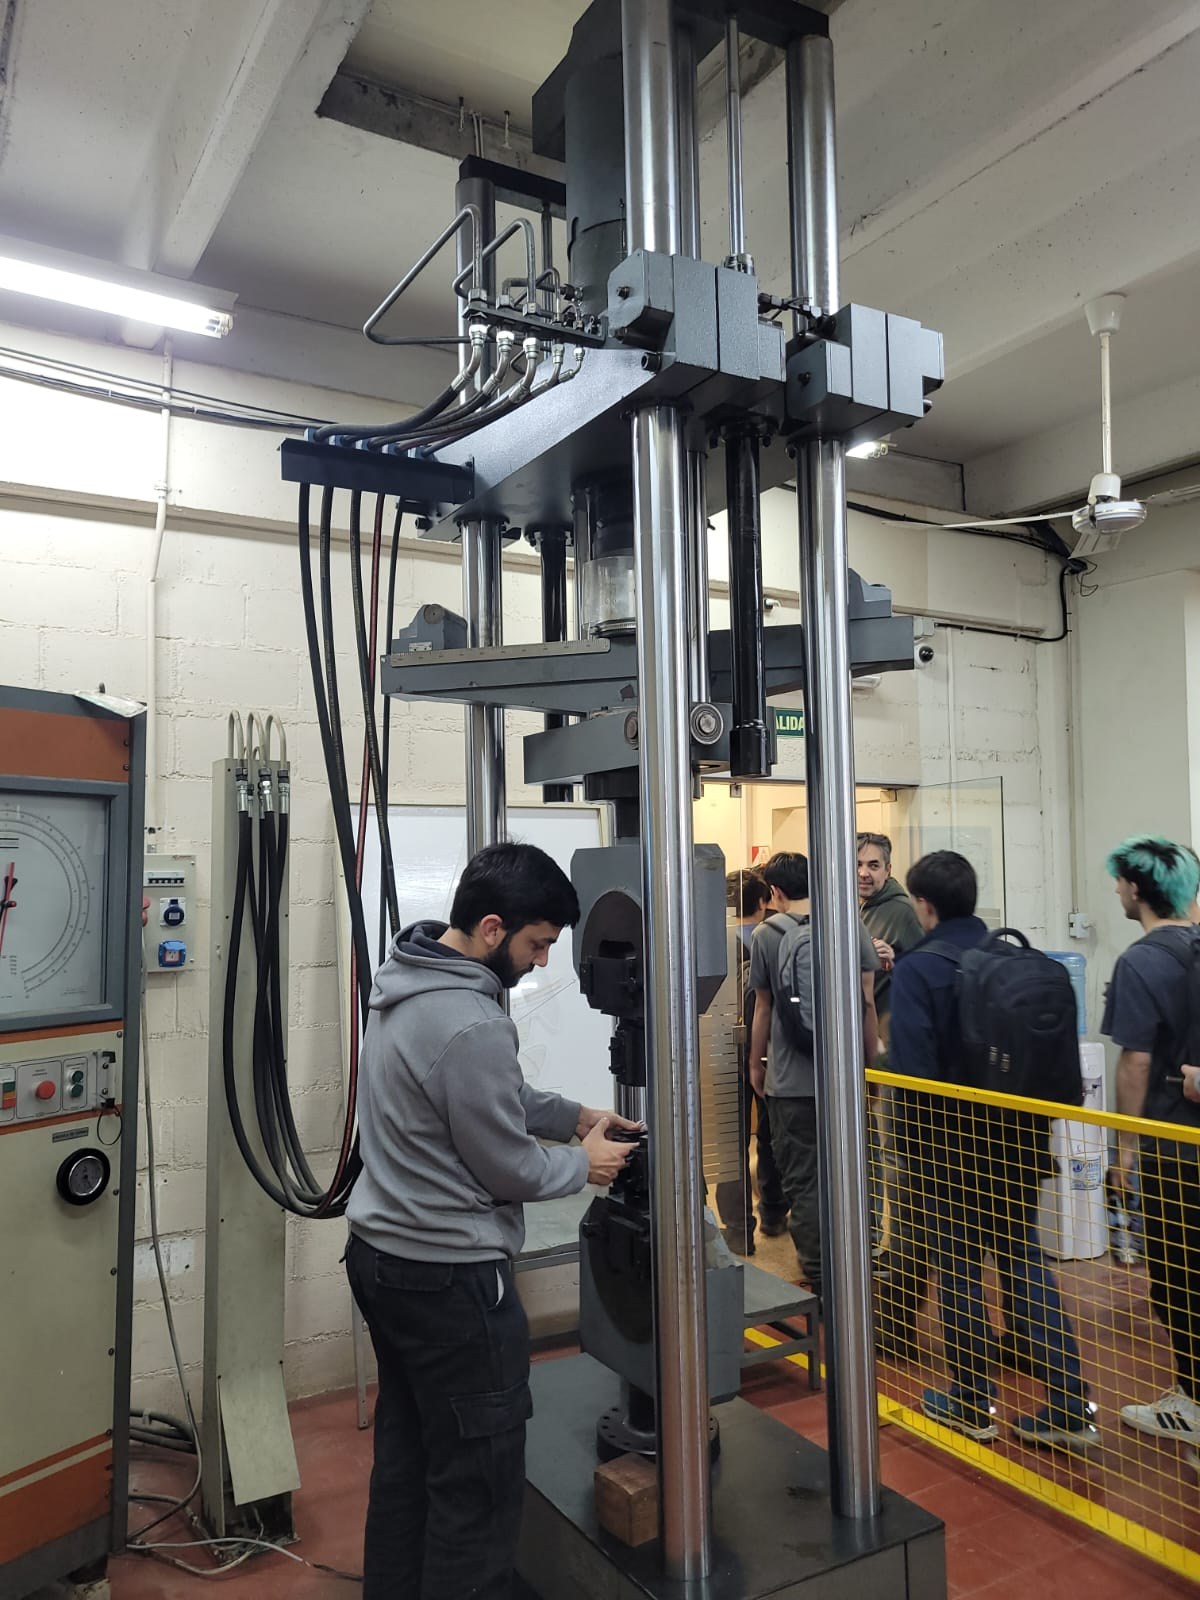
\includegraphics[width=0.55\textwidth]{images/maquina_universal_ensayos.jpeg}
    \caption{Máquina universal de ensayos de tracción y compresión relevada en laboratorio.}
    \label{fig.ej1:maquina_universal}
\end{figure}

Para la adquisición y caracterización completa de un ensayo mecánico se requiere registrar en tiempo real dos variables
físicas fundamentales: la fuerza axial aplicada (o carga) y la deformación longitudinal (o desplazamiento) de la
mordaza móvil respecto a la fija.

\subsection{Identificación y Especificaciones de los Sensores}
A partir de la inspección física y el registro fotográfico se relevaron dos transductores industriales montados
directamente sobre la máquina:
\begin{enumerate}
    \item \emph{Transductor de Posición Lineal (GEFRAN)}: Corresponde a un potenciómetro
    lineal de precisión marca GEFRAN modelo PY-2-C-100 (Figura~\ref{fig.ej1:gefran}(b) y
    hoja de datos~\cite{gefran_py2} adjunta en el Anexo~\ref{ch:anexos}), con resistencia nominal total de
    $\qty{5}{\kilo\ohm}\pm 20\%$, carrera eléctrica útil de $\qty{100}{\milli\meter}$ (carrera teórica de $\qty{101}{\milli\meter}$,
    mecánica de $\qty{106}{\milli\meter}$). La tecnología de pista plástica
    conductora provee una resolución teórica infinita y una excelente linealidad independiente garantizada de
    $\pm 0.07\%$. La hoja de datos sugiere que el dispositivo opere en configuración
    ratiométrica con una corriente de cursor $I_c \le \qty{0.1}{\milli\ampere}$ ($< \qty{0.1}{\micro\ampere}$ recomendado)
    para no degradar la linealidad ni el ciclo de vida ($> 25 \times 10^6\unit{\meter}$ de carrera), aspecto clave que
    fundamenta el diseño del circuito de acondicionamiento.
    \item \emph{Transmisor de Presión Hidráulica (ADZ NAGANO)}: Instalado en la línea hidráulica principal de
    alimentación del pistón de carga (ver Figura~\ref{fig.ej1:adz}(a)). La placa de características
    técnicas del dispositivo (ver Figura~\ref{fig.ej1:adz}(b) y hoja de datos~\cite{adz_nagano} adjunta en el
    Anexo~\ref{ch:anexos}) certifica su procedencia de ADZ NAGANO Sensortechnik GmbH, serie industrial SML (tipo SML-10.0),
    con rango calibrado de $\qtyrange{0}{250}{\bar}$, sobrepresión admisible de $\qty{750}{\bar}$, presión de rotura de
    $\qty{1000}{\bar}$, tensión de alimentación de $\qtyrange{12}{32}{\volt}$~DC y salida analógica en tensión de
    $\qtyrange{0}{10}{\volt}$ (3 hilos, tiempo de respuesta $\le \qty{1}{\milli\second}$, clase de exactitud $\le 0.5\%$).
    Sabiendo que la fuerza ejercida por el pistón es el
    producto directo de la presión hidráulica por el área de su sección transversal ($F = P \cdot A_{\text{pistón}}$),
    la medición unificada de presión permite determinar la carga con exactitud.
\end{enumerate}

\begin{figure}[!ht]
    \centering
    \begin{subfigure}[t]{0.48\textwidth}
        \centering
        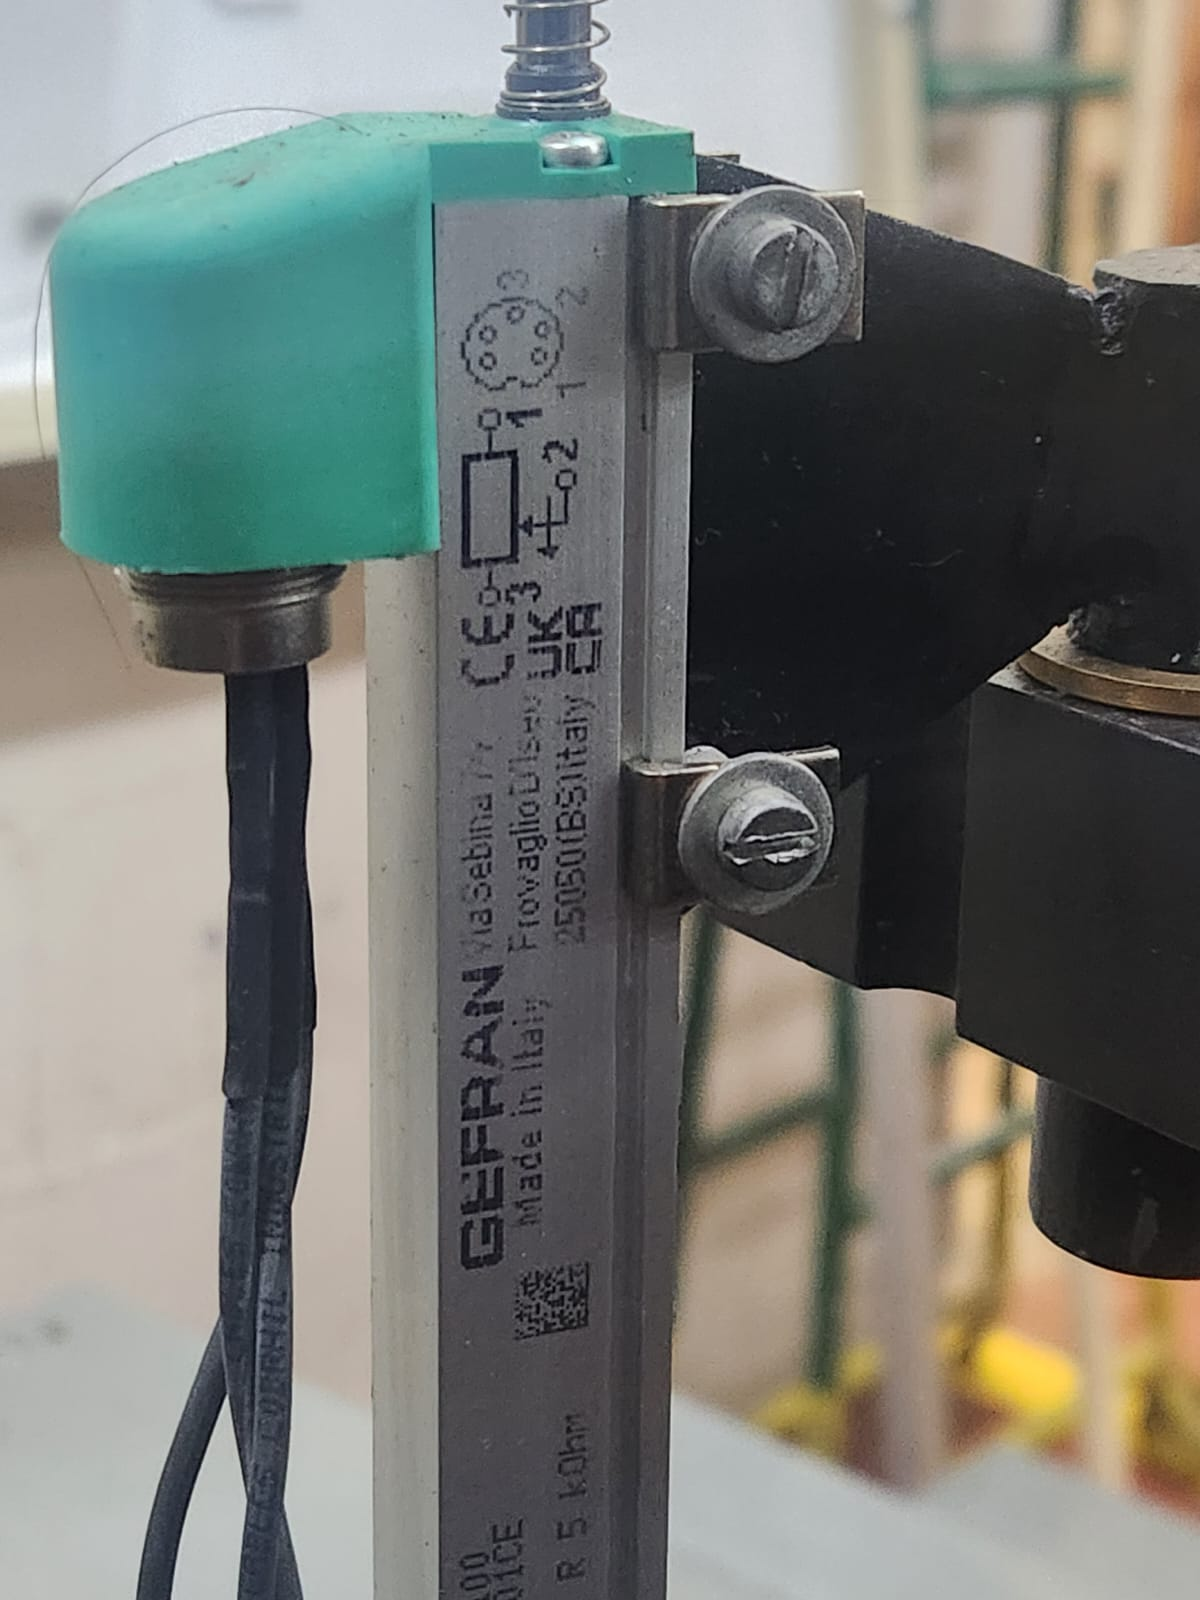
\includegraphics[width=\textwidth]{images/foto_transductor_gefran.jpg}
        \caption{Montaje de transductor GEFRAN.}
        \label{fig.ej1:gefran_montaje}
    \end{subfigure}
    \hfill
    \begin{subfigure}[t]{0.48\textwidth}
        \centering
        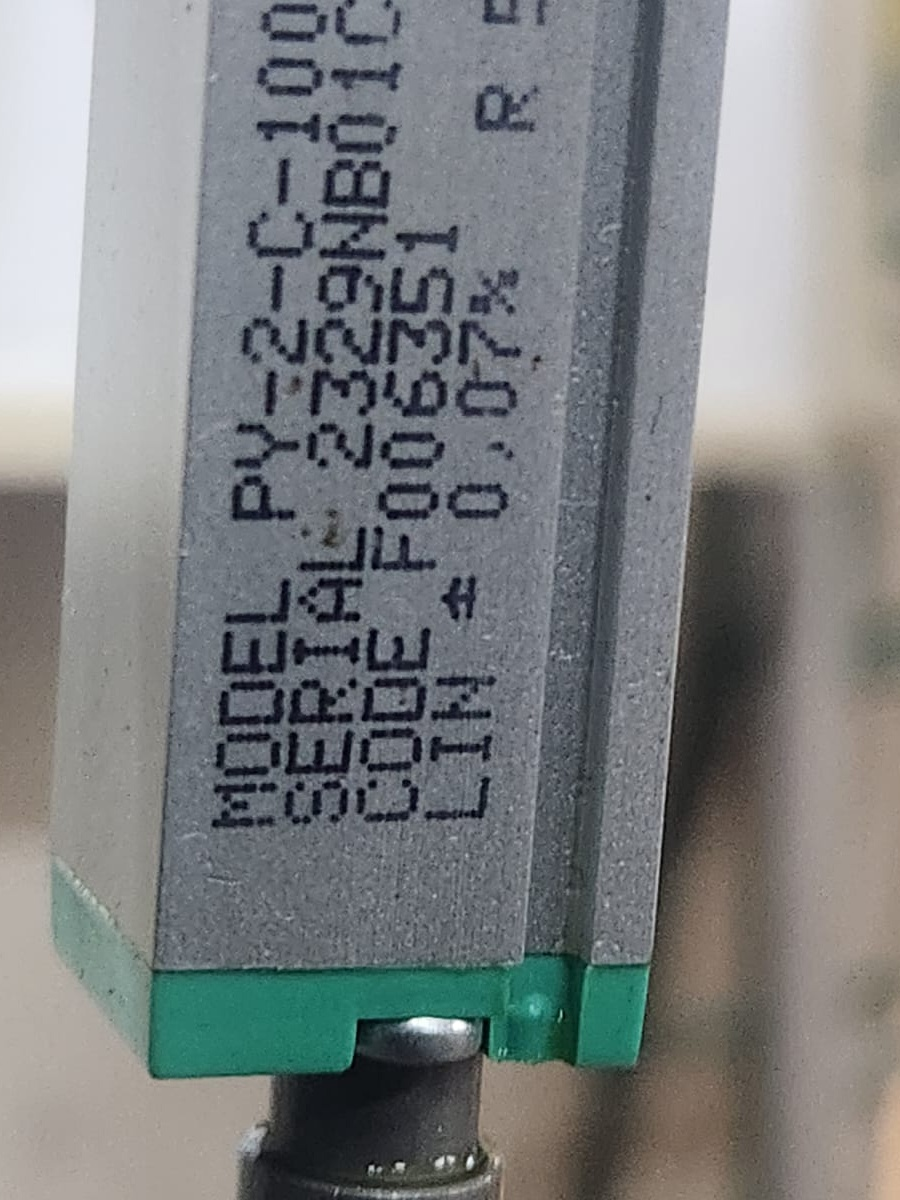
\includegraphics[width=\textwidth]{images/modelo_sensor_desplazamiento_crop.jpeg}
        \caption{Modelo GEFRAN PY-2-C-100.}
        \label{fig.ej1:gefran_modelo}
    \end{subfigure}
    \caption{Transductor potenciométrico de posición lineal GEFRAN relevado.}
    \label{fig.ej1:gefran}
\end{figure}

\begin{figure}[!ht]
    \centering
    \begin{subfigure}[t]{0.48\textwidth}
        \centering
        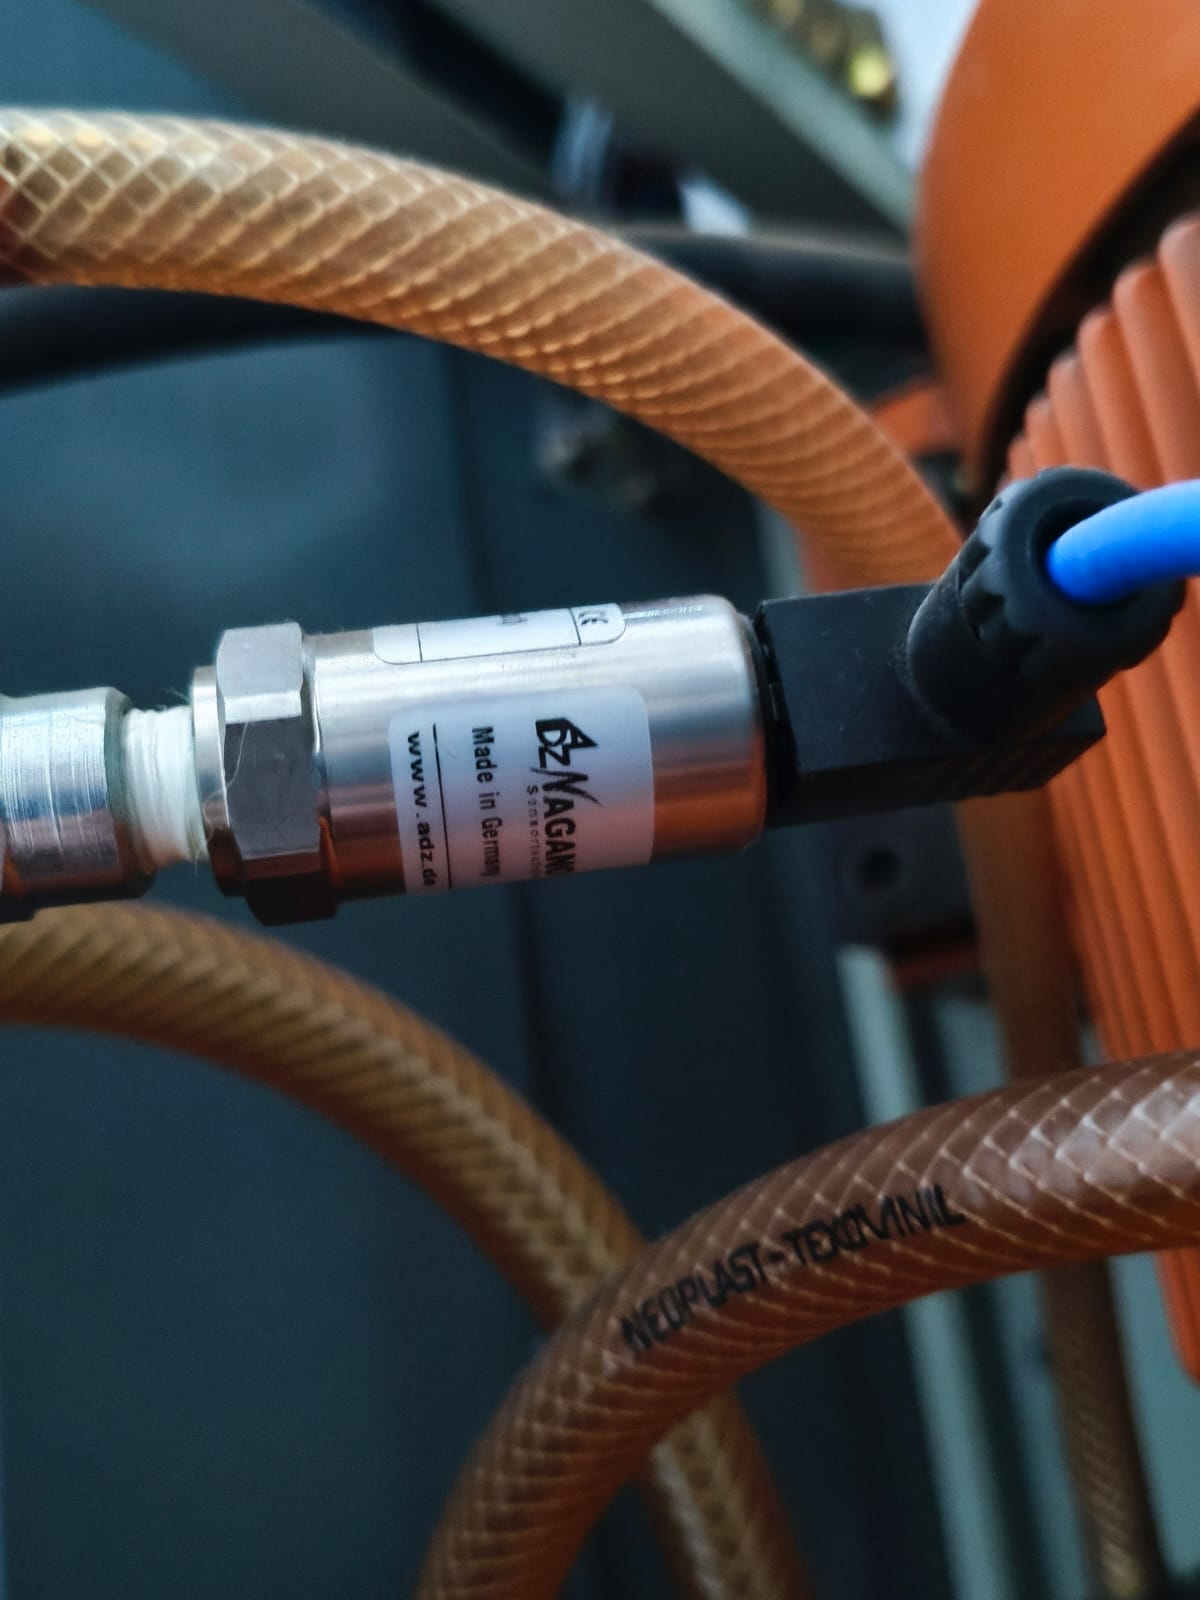
\includegraphics[width=\textwidth]{images/foto_transductor_adz_1.jpg}
        \caption{Transmisor ADZ NAGANO (marca y conector).}
        \label{fig.ej1:adz_montaje}
    \end{subfigure}
    \hfill
    \begin{subfigure}[t]{0.48\textwidth}
        \centering
        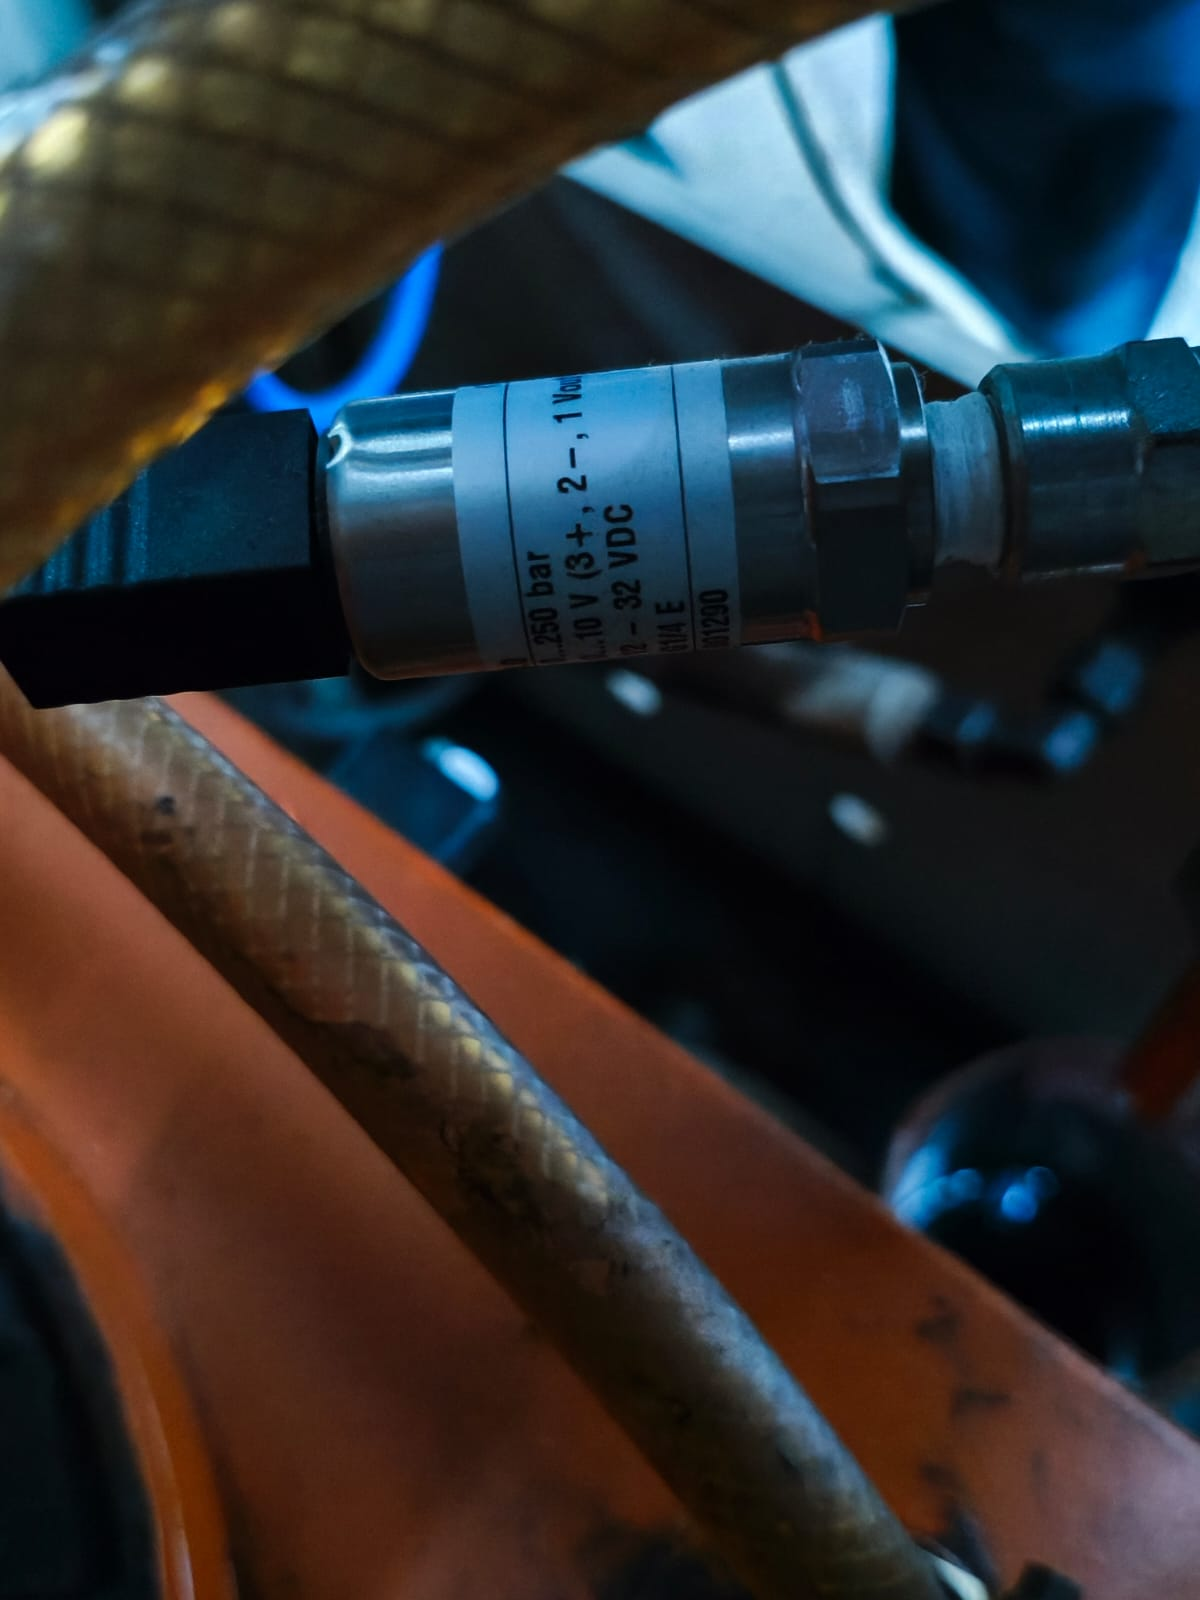
\includegraphics[width=\textwidth]{images/sensor_presion_specs.jpeg}
        \caption{Placa de características técnicas del sensor ADZ.}
        \label{fig.ej1:adz_specs}
    \end{subfigure}
    \caption{Transmisor de presión hidráulica industrial ADZ NAGANO relevado.}
    \label{fig.ej1:adz}
\end{figure}

\subsection{Selección del Sistema Embebido y Especificaciones del Conversor ADC}
La consigna de este trabajo práctico establece como requisitos de diseño alcanzar una precisión de resolución mínima de
$\Delta x \le \qty{0.1}{\milli\meter}$ en el desplazamiento y $\Delta M \le \qty{15}{\kilogram}$ en la carga. A partir de
estas exigencias metrológicas y de las características de los sensores relevados, se definen los parámetros del sistema
de digitalización y control:
\begin{enumerate}
    \item \emph{Resolución del ADC para Desplazamiento}: Para una carrera total de $L = \qty{100}{\milli\meter}$ y un
    escalón requerido de $\qty{0.1}{\milli\meter}$, el número de divisiones mínimas es:
    \[
        N_x = \frac{\qty{100}{\milli\meter}}{\qty{0.1}{\milli\meter}} = 1000\text{ niveles}
    \]
    Un conversor de 10 bits dispone de $2^{10} = 1024$ niveles, logrando una resolución teórica de
    $\frac{\qty{100}{\milli\meter}}{1024} \approx \qty{0.0977}{\milli\meter}$, lo que apenas satisface el umbral
    nominal sin margen de ruido. Al seleccionar un ADC de 12 bits ($2^{12} = 4096$ niveles), la resolución del
    sistema pasa a ser:
    \[
        \Delta x_{\text{cuanta}} = \frac{\qty{100}{\milli\meter}}{4096} \approx \qty{0.0244}{\milli\meter}
    \]
    Este margen ($4\times$) absorbe holgadamente las fluctuaciones por ruido y garantiza el cumplimiento aun
    cuando la cantidad efectiva de bits (ENOB) sea de $10.5\text{ bits}$.
    \item \emph{Resolución del ADC para Carga / Fuerza}: Considerando una máquina hidráulica con capacidad máxima de
    $\qty{20000}{\kilogram}$, la exigencia de $\Delta M \le \qty{15}{\kilogram}$ requiere:
    \[
        N_F = \frac{\qty{20000}{\kilogram}}{\qty{15}{\kilogram}} \approx 1333.3\text{ niveles}
    \]
    Con un conversor de 12 bits ($4096$ cuentas a escala completa), aun reservando un margen de escala superior
    preventivo del orden del $12\%$ en la etapa analógica para absorber sobrepresiones transitorias sin
    saturar el conversor ($\approx 3650$ cuentas efectivas correspondientes a la salida nominal), la resolución teórica
    resultante es:
    \[
        \Delta M_{\text{cuanta}} = \frac{\qty{20000}{\kilogram}}{3650} \approx \qty{5.48}{\kilogram}
    \]
    satisfaciendo ampliamente la especificación requerida ($\qty{5.48}{\kilogram} \ll \qty{15}{\kilogram}$).
    \item \emph{Frecuencia de Muestreo ($f_s$)}: Los ensayos de tracción son fenómenos mecánicos cuasi-estáticos con
    velocidades de desplazamiento de $\qtyrange{1}{20}{\milli\meter/\minute}$, donde el espectro útil de la señal no
    sobrepasa los $\qty{2}{\hertz}$. Fijando una frecuencia de muestreo de $f_s = \qty{100}{\text{S/s}}$
    ($\qty{100}{\hertz}$), se cumple sobradamente el criterio de Nyquist-Shannon y se dispone de un
    sobremuestreo de $25\times$, posibilitando la aplicación de promediado digital móvil (\emph{moving
    average}) para suprimir el rizado de $\qty{50}{\hertz}$.
    \item \emph{Sistema Embebido Seleccionado}: Se adopta el microcontrolador STM32F103C8T6 con núcleo ARM Cortex-M3 a
    $\qty{72}{\mega\hertz}$ (habitual en placas de desarrollo tipo \emph{Blue Pill}). El chip incorpora dos conversores ADC SAR de 12 bits integrados, temporizadores para el disparo equidistante de muestreo mediante DMA e interfaz USB 2.0 nativa (clase CDC virtual COM) para el envío directo de tramas a la computadora de ensayo.
\end{enumerate}

\subsection{Diseño del Circuito de Acondicionamiento Analógico}
Habiendo establecido que la etapa de digitalización se basará en el conversor ADC de 12 bits del microcontrolador
STM32F103C8T6, con una tensión de referencia estabilizada de $V_{\text{ref}} = \qty{3.300}{\volt}$ (rango de entrada
$\qtyrange{0}{3.3}{\volt}$) y una tasa de muestreo de $f_s = \qty{100}{\text{S/s}}$, se procede al diseño de las
etapas de adaptación analógica para cada transductor:
\begin{itemize}
    \item \emph{Canal de Posición (GEFRAN)}: El potenciómetro se polariza directamente con la tensión de referencia estabilizada del microcontrolador ($V_{\text{ref}} = \qty{+3.3}{\volt}$), de modo que la tensión en el cursor varía linealmente entre $\qty{0}{\volt}$ y $\qty{3.3}{\volt}$. Esta elección de alimentación no presenta inconvenientes y ofrece ventajas técnicas determinantes:
    \begin{enumerate}
        \item \emph{Medición estrictamente ratiométrica}: Al compartir la misma tensión de referencia tanto la excitación del potenciómetro como el conversor ADC, cualquier fluctuación o deriva térmica en la fuente se cancela. De este modo, la conversión resulta inmune a variaciones de alimentación sin depender de la exactitud absoluta de la tensión de referencia.
        \item \emph{Autocalentamiento despreciable}: Para una resistencia nominal de $\qty{5}{\kilo\ohm}$, la disipación sobre la pista plástica es de apenas:
        \[
            P = \frac{(\qty{3.3}{\volt})^2}{\qty{5}{\kilo\ohm}} \approx \qty{2.18}{\milli\watt}
        \]
        Este valor representa menos del $0.1\%$ de la potencia máxima admisible especificada por el fabricante ($\qty{2.4}{\watt}$), garantizando que no se introduzcan derivas resistivas por calentamiento local del transductor.
        \item \emph{Sensibilidad y resolución adecuadas}: Con una excursión de $\qty{3.3}{\volt}$ a lo largo de los $\qty{100}{\milli\meter}$ de carrera útil, la sensibilidad del sensor es de $\qty{33}{\milli\volt\per\milli\meter}$. El escalón correspondiente a la resolución mínima exigida de $\Delta x = \qty{0.1}{\milli\meter}$ es de $\Delta V = \qty{3.3}{\milli\volt}$, lo que equivale a unas 4 cuentas en un ADC de 12 bits ($1\,\text{LSB} \approx \qty{0.806}{\milli\volt}$), superando holgadamente el piso de ruido térmico.
    \end{enumerate}
    Para respetar rigurosamente la recomendación de la hoja de datos de mantener
        una corriente de cursor despreciable ($I_c \ll
        \qty{0.1}{\micro\ampere}$) y anular cualquier error de carga sobre la
        pista resistiva, se interpone un amplificador operacional en
        configuración de seguidor de tensión (buffer con ganancia unitaria $G =
        1$) que presenta una impedancia de entrada elevada. A la salida del buffer se implementa un filtro pasabajos RC anti-aliasing pasivo de primer orden con resistencia $R_f = \qty{1}{\kilo\ohm}$ y capacitor cerámico $C_f = \qty{100}{\nano\farad}$, fijando una frecuencia de corte teórica según la Ecuación~\ref{eq.ej1:filtro_fc}:
    \begin{equation}
        f_c = \frac{1}{2 \pi R_f C_f}
        \label{eq.ej1:filtro_fc}
    \end{equation}
    Calculando con los valores adoptados, resulta:
    \[
        f_c = \frac{1}{2 \pi \cdot \qty{1}{\kilo\ohm} \cdot \qty{100}{\nano\farad}} \approx \qty{1.59}{\kilo\hertz}
    \]
    \item \emph{Canal de Presión (ADZ NAGANO)}: La salida analógica del sensor entrega $\qtyrange{0}{10}{\volt}$, mientras que el ADC del microcontrolador trabaja con una referencia de $\qty{3.3}{\volt}$ y no tolera tensiones superiores a $V_{\text{DDA}} + \qty{0.3}{\volt}$. Por ello, se emplea un divisor resistivo de precisión para atenuar la señal y, para evitar saturación del ADC ante sobrepresiones hidráulicas o transitorios de bombeo y proteger el pin analógico, se diseña el divisor con un margen superior.

    Empleando resistores de película metálica de precisión al $0.1\%$ con valores normalizados de $R_1 = \qty{24}{\kilo\ohm}$ y $R_2 = \qty{10}{\kilo\ohm}$, la ganancia del divisor resulta:
    \begin{equation}
        G = \frac{R_2}{R_1 + R_2} = \frac{\qty{10}{\kilo\ohm}}{\qty{24}{\kilo\ohm} + \qty{10}{\kilo\ohm}} = \frac{10}{34} \approx 0.2941
        \label{eq.ej1:divisor_presion}
    \end{equation}
    Bajo esta relación:
    \begin{itemize}
        \item Para la salida nominal máxima de $\qty{10}{\volt}$ ($\qty{250}{\bar}$), la tensión atenuada es de $\qty{2.941}{\volt}$, asegurando que la señal permanezca dentro del rango lineal del ADC ($V_{\text{ref}} = \qty{3.300}{\volt}$).
        \item La impedancia de carga total que presenta el divisor al transmisor es $R_{\text{carga}} = R_1 + R_2 = \qty{34}{\kilo\ohm}$, satisfaciendo con amplio margen la especificación de carga mínima exigida por el fabricante ($R_L \ge \qty{4.7}{\kilo\ohm}$).
    \end{itemize}
    La señal atenuada se acopla a un seguidor de tensión con filtro pasabajos idéntico antes de ingresar al canal del ADC.
\end{itemize}

El esquema eléctrico del circuito de acondicionamiento propuesto se presenta en la
Figura~\ref{crkt.ej1:acondicionamiento}.

\begin{figure}[!ht]
    \centering
    \begin{tikzpicture}[scale=0.85, transform shape]
    % Canal 1: Potenciometro Lineal
    \node[anchor=west, font=\bfseries] at (-1, 3.8) {Canal 1: Posición (GEFRAN)};
    \draw (-1, 2.5) node[left] {$+3.3\V$} to[short, o-] (0.5, 2.5)
          to[pR, name=pot, l_={$R_p$ ($5\kohm$)}] (0.5, 0.5)
          to[short, -o] (-1, 0.5) node[left] {GND};
    
    \draw (pot.wiper) to[short] (2.0, 1.5)
          node[op amp, anchor=+](op1){};
    \draw (op1.-) -- ++(-0.2, 0) -- ++(0, 0.8) -| ($(op1.out) + (0.3, 0)$) coordinate(out1);
    \draw (op1.out) to[short] (out1)
          to[R, l={$R_f$ ($1\kohm$)}, *-*] ++(2.5, 0) coordinate(flt1)
          to[short, -o] ++(1.8, 0) node[right] {ADC CH1 ($0\dots 3.3\V$)};
    \draw (flt1) to[C, l={$C_f$ ($100\nF$)}, -*] ++(0, -1.4) node[ground]{};

    % Canal 2: Presion Hidraulica
    \node[anchor=west, font=\bfseries] at (-1, -1.0) {Canal 2: Presión (ADZ NAGANO)};
    \draw (-1, -3.2) node[left] {$V_{\text{in}}\text{ (}0\dots 10\V\text{)}$} to[short, o-] (0.5, -3.2)
          to[R, l={$R_1$ ($24\kohm$)}, -*] (2.2, -3.2) coordinate(div2)
          to[R, l_={$R_2$ ($10\kohm$)}, *-*] ++(0, -2.0) node[ground]{};
    
    \draw (div2) to[short] (3.4, -3.2)
          node[op amp, anchor=+](op2){};
    \draw (op2.-) -- ++(-0.2, 0) -- ++(0, 0.7) -| ($(op2.out) + (0.3, 0)$) coordinate(out2);
    \draw (op2.out) to[short] (out2)
          to[R, l={$R_f$ ($1\kohm$)}, *-*] ++(2.5, 0) coordinate(flt2)
          to[short, -o] ++(1.8, 0) node[right] {ADC CH2 ($0\dots 3.3\V$)};
    \draw (flt2) to[C, l={$C_f$ ($100\nF$)}, -*] ++(0, -1.4) node[ground]{};
\end{tikzpicture}

    \caption{Esquema eléctrico de acondicionamiento analógico para la máquina de tracción.}
    \label{crkt.ej1:acondicionamiento}
\end{figure}

En la Figura~\ref{fig.ej1:diagrama_bloques} se resume el diagrama en bloques funcional del sistema completo de
instrumentación y adquisición de datos propuesto para la máquina universal de ensayos.

\begin{figure}[!ht]
    \centering
    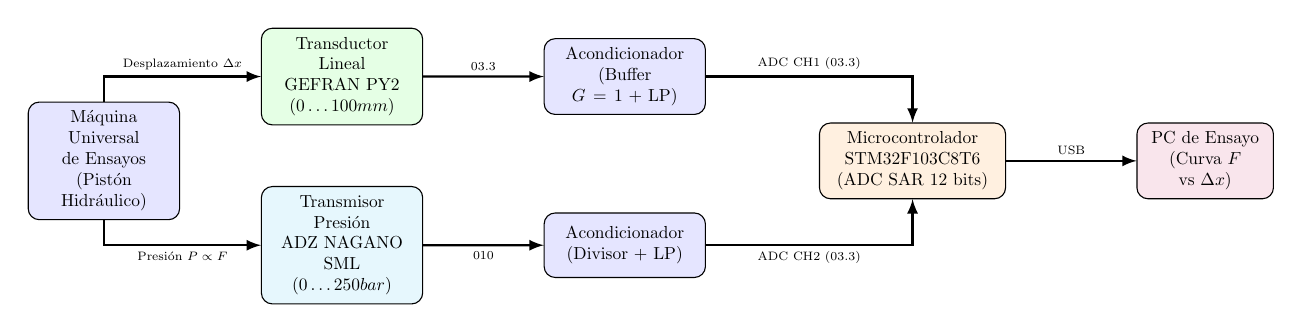
\begin{tikzpicture}[scale=0.63, transform shape,
    block/.style={rectangle, draw, fill=blue!10, text width=2.9cm, text centered,
                  rounded corners, minimum height=1.3cm, inner sep=5pt},
    line/.style={draw, -latex, thick}]

    % Sistema Mecanico (Fuente)
    \node [block, text width=2.7cm] (maquina) at (0, 0) {Máquina Universal\\de Ensayos\\(Pistón Hidráulico)};

    % Canal 1: Posicion / Desplazamiento
    \node [block, fill=green!10, text width=2.9cm] (gefran) at (4.8, 1.7) {Transductor Lineal\\GEFRAN PY2\\($0\dots 100\unit{mm}$)};
    \node [block, text width=2.9cm] (acond1) at (10.5, 1.7) {Acondicionador\\(Buffer $G=1$ + LP)};

    % Canal 2: Presion / Carga
    \node [block, fill=cyan!10, text width=2.9cm] (adz) at (4.8, -1.7) {Transmisor Presión\\ADZ NAGANO SML\\($0\dots 250\unit{bar}$)};
    \node [block, text width=2.9cm] (acond2) at (10.5, -1.7) {Acondicionador\\(Divisor + LP)};

    % Sistema Embebido y PC
    \node [block, fill=orange!12, text width=3.4cm] (mcu) at (16.3, 0) {Microcontrolador\\STM32F103C8T6\\(ADC SAR 12 bits)};
    \node [block, fill=purple!10, text width=2.4cm] (pc) at (22.2, 0) {PC de Ensayo\\(Curva $F$ vs $\Delta x$)};

    % Rutas y flechas
    \path [line] (maquina.north) -- (maquina.north |- gefran.west) -- node[above, midway, font=\scriptsize] {Desplazamiento $\Delta x$} (gefran.west);
    \path [line] (maquina.south) -- (maquina.south |- adz.west) -- node[below, midway, font=\scriptsize] {Presión $P \propto F$} (adz.west);

    \path [line] (gefran) -- node[above, midway, font=\scriptsize] {$\qtyrange{0}{3.3}{\volt}$} (acond1);
    \path [line] (adz) -- node[below, midway, font=\scriptsize] {$\qtyrange{0}{10}{\volt}$} (acond2);

    \path [line] (acond1.east) -- node[above, midway, font=\scriptsize] {ADC CH1 ($\qtyrange{0}{3.3}{\volt}$)} (acond1.east -| mcu.north) -- (mcu.north);
    \path [line] (acond2.east) -- node[below, midway, font=\scriptsize] {ADC CH2 ($\qtyrange{0}{3.3}{\volt}$)} (acond2.east -| mcu.south) -- (mcu.south);

    \path [line] (mcu) -- node[above, midway, font=\scriptsize] {USB} (pc);
\end{tikzpicture}

    \caption{Diagrama en bloques del sistema de instrumentación y adquisición para la máquina universal de ensayos.}
    \label{fig.ej1:diagrama_bloques}
\end{figure}

\clearpage

\section{Experimento 2: Sistema de Instrumentación para Banco de Motores de Combustión}

\subsection{Fundamentos del Banco de Ensayo y Principio de Medición}
El ensayo de motores de combustión interna en banco dinamométrico permite trazar las curvas características de par motor
y potencia efectiva en función del régimen de giro~\cite{barreiro_banco}. El equipamiento del laboratorio corresponde a
un \emph{banco de motor de acople directo} (ver Figura~\ref{fig.ej2:banco_motor}), donde el volante de inercia se une
directamente al freno sobre una bancada rígida. Al ensayar el motor fuera del vehículo, se evalúa su potencia neta sin
las pérdidas parásitas por fricción en la transmisión y rodadura de neumáticos inherentes a los bancos de
rodillos~\cite{barreiro_banco}.

\begin{figure}[!ht]
    \centering
    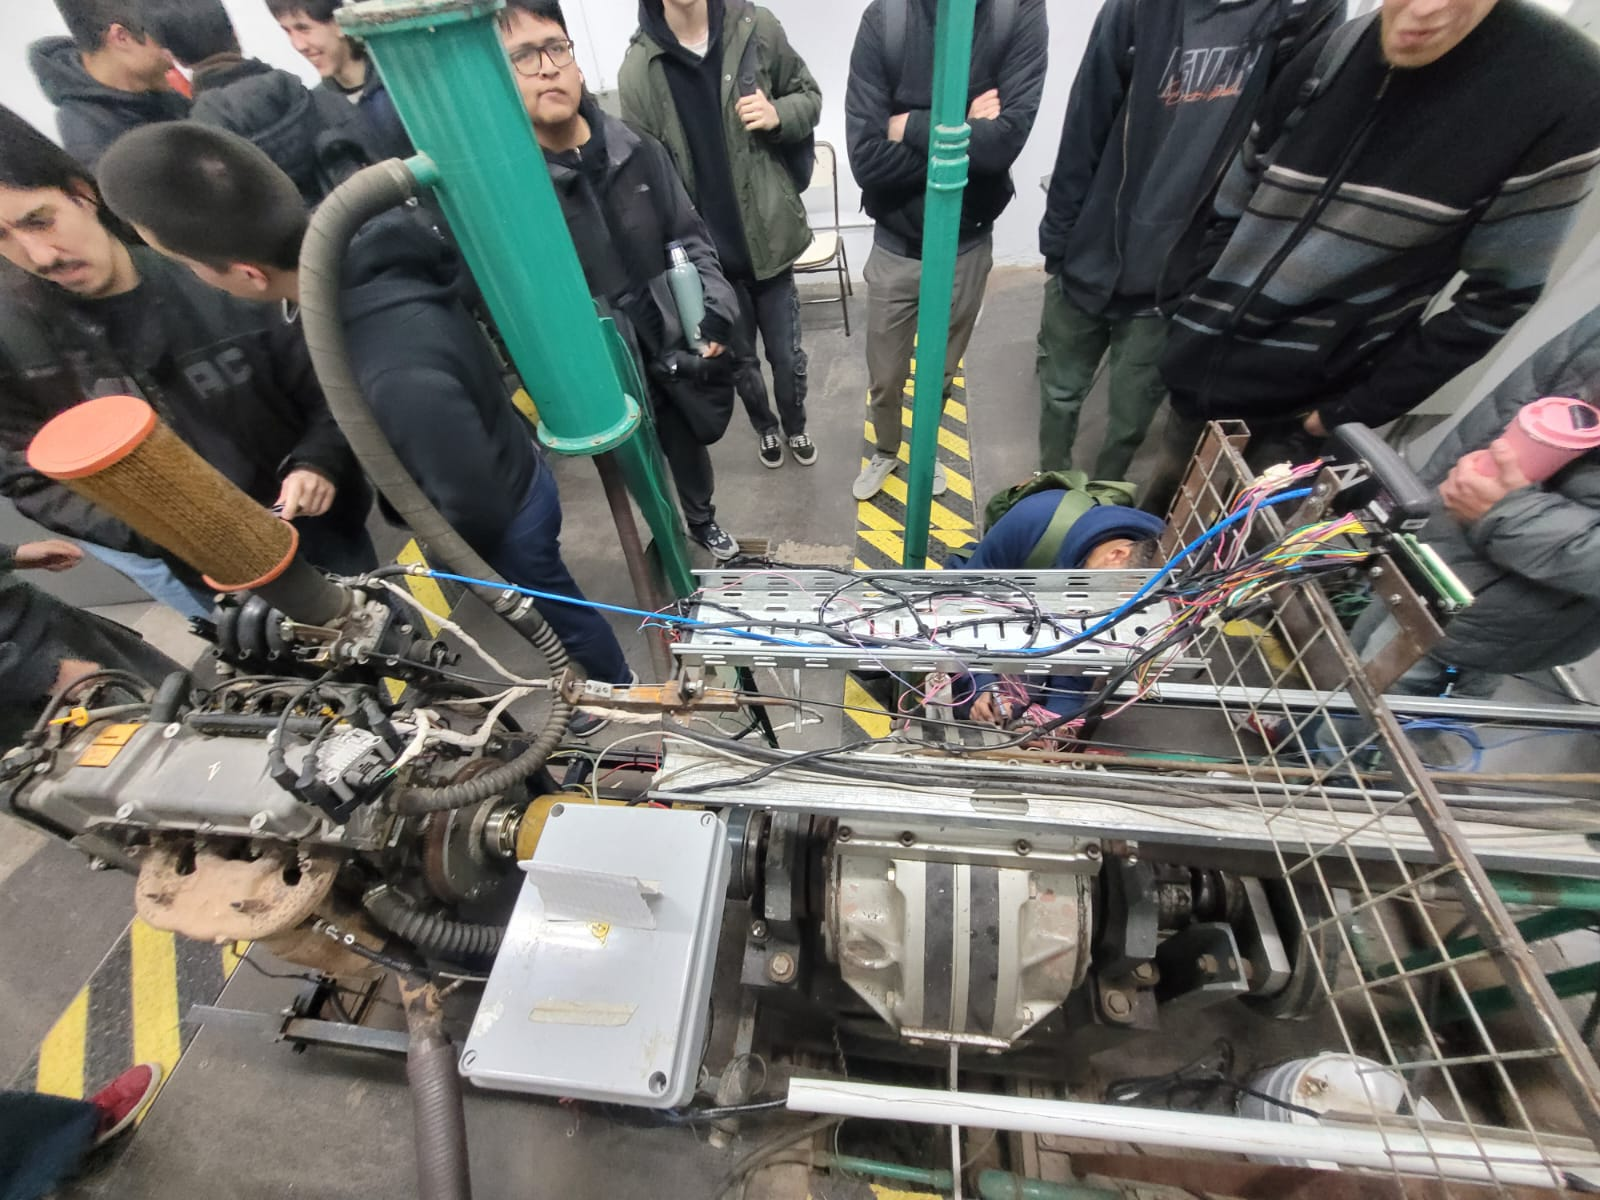
\includegraphics[width=0.65\textwidth]{images/banco_prueba_motor.jpeg}
    \caption{Banco dinamométrico para ensayo de motores de combustión interna relevado en laboratorio.}
    \label{fig.ej2:banco_motor}
\end{figure}

A diferencia de los bancos inerciales (que sólo operan en aceleración transitoria libre), este equipo utiliza un freno
dinamométrico de absorción (hidráulico o de corrientes parásitas) que disipa la potencia generada, permitiendo estabilizar
al motor a RPM constantes. Para una medición confiable es indispensable ensayar en \emph{régimen estacionario}, ya que
en aceleración parte de la potencia se destina a acelerar las masas inerciales internas (cigüeñal y volante), lo que
subestimaría el par efectivo transferido al freno~\cite{barreiro_banco}.

Por la tercera ley de Newton (acción y reacción), el estator del freno bascula sobre cojinetes libres y transmite el par
a una celda de carga montada sobre un brazo de palanca de longitud $L$. El par motor $\tau$ y la potencia al freno $P$ se
calculan analíticamente según:
\begin{equation}
    \tau = F \cdot L = m_{\text{medida}} \cdot g \cdot L
    \label{eq.ej2:torque}
\end{equation}
\begin{equation}
    P = \tau \cdot \omega = \tau \cdot \frac{2 \pi N}{60}
    \label{eq.ej2:potencia}
\end{equation}
donde $N$ es la velocidad angular en RPM. Antes de los ensayos, la celda de carga se calibra estáticamente verificando el
cero en reposo y suspendiendo masas patrón en el brazo de palanca ($\tau_{\text{patrón}} = M_{\text{patrón}} \cdot g \cdot L$).

\subsection{Sensores Relevados en el Banco}
A partir del relevamiento in situ en el laboratorio se identificaron los dos transductores primarios de la máquina
(ver Figura~\ref{fig.ej2:transductores}):
\begin{enumerate}
    \item \emph{Celda de Carga Dinamométrica}: Montada en el brazo oscilante del freno (ver Figura~\ref{fig.ej2:transductores}(a)).
    Es un transductor de precisión tipo \emph{S-beam} con puente de Wheatstone de cuatro galgas extensométricas ($\qty{350}{\ohm}$,
    sensibilidad de $\qty{3}{\milli\volt\per\volt}$) que genera una tensión diferencial en milivoltios proporcional a la
    fuerza del estator.
    \item \emph{Sensor de Efecto Hall para RPM}: Montado de forma fija frente a una rueda fónica dentada acoplada al eje
    (ver Figura~\ref{fig.ej2:transductores}(b)). Al girar el motor, genera una señal digital de pulsos cuya frecuencia es
    proporcional a la velocidad de giro ($f_{\text{pulsos}} = Z \cdot \frac{N}{60}$, con $Z$ dientes), eliminando el desgaste
    mecánico y tolerando las vibraciones del banco.
\end{enumerate}

\begin{figure}[!ht]
    \centering
    \begin{subfigure}[t]{0.48\textwidth}
        \centering
        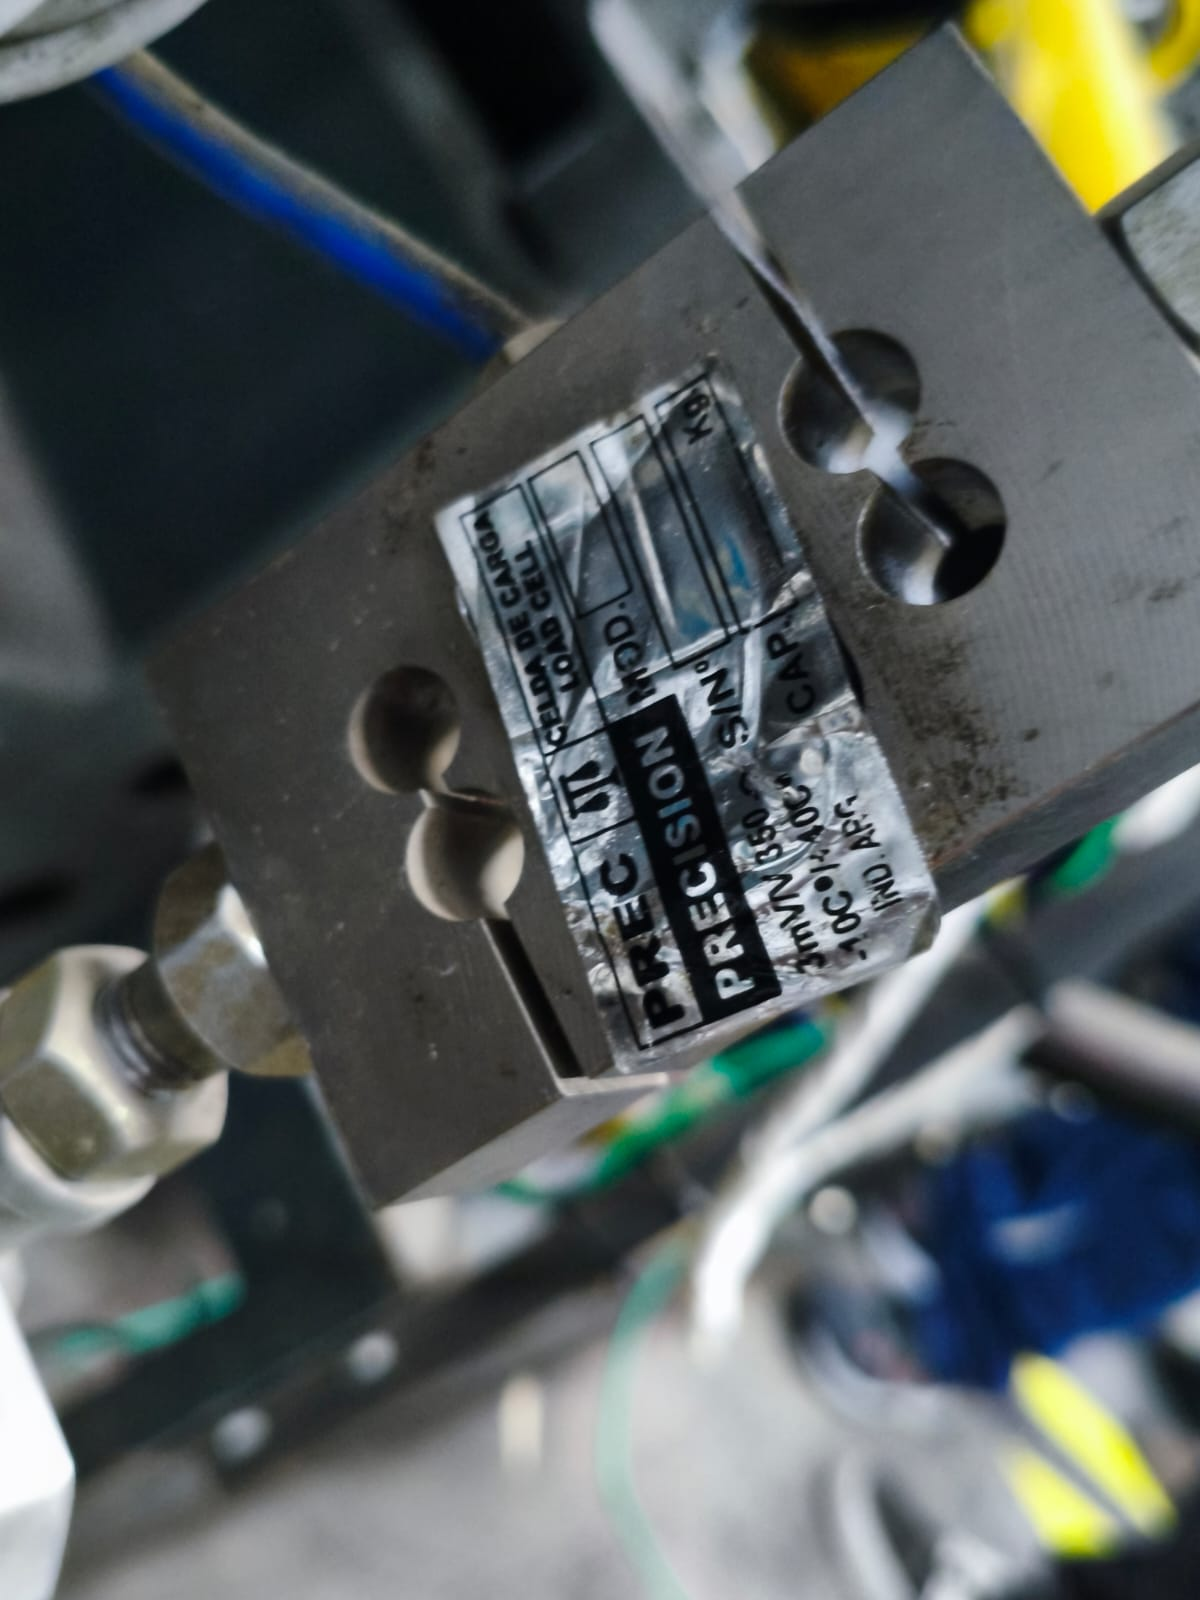
\includegraphics[width=\textwidth]{images/ej2_celda_carga.jpeg}
        \caption{Celda de carga tipo S-beam montada en el brazo.}
        \label{fig.ej2:celda_carga}
    \end{subfigure}
    \hfill
    \begin{subfigure}[t]{0.48\textwidth}
        \centering
        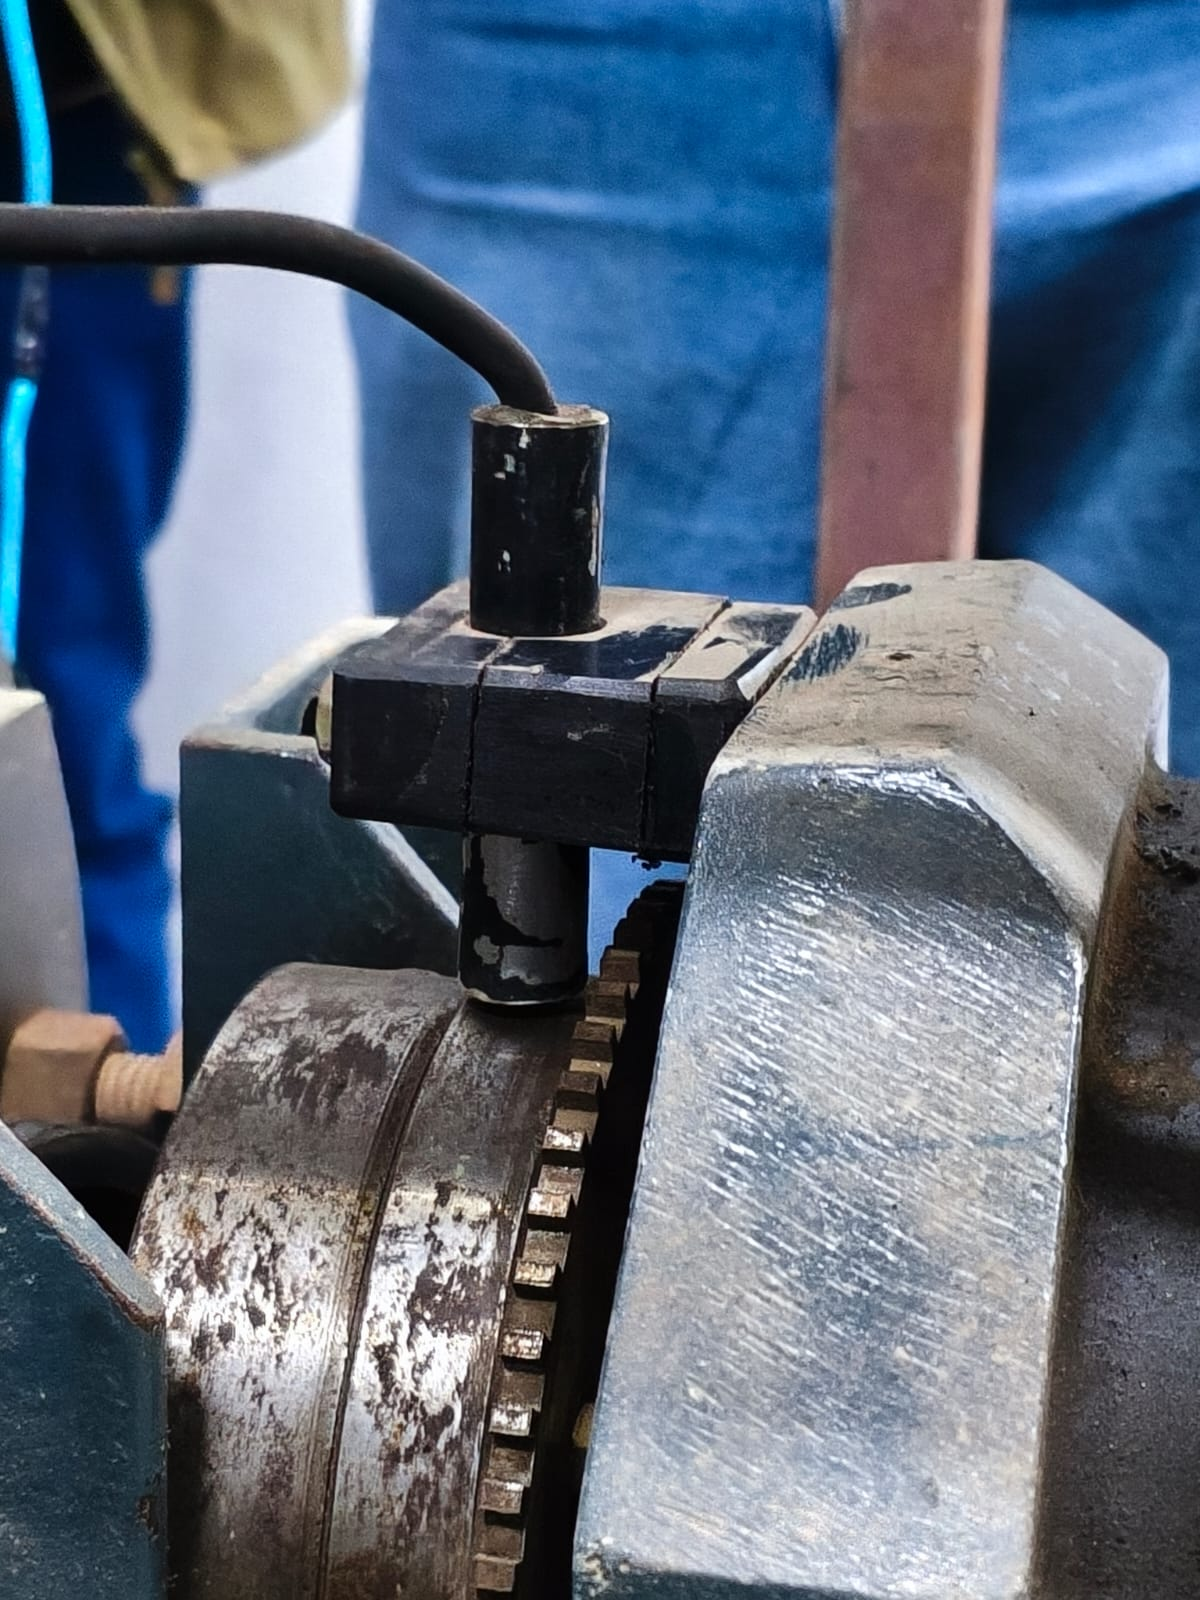
\includegraphics[width=\textwidth]{images/ej2_sensor_hall.jpeg}
        \caption{Sensor de efecto Hall enfrentado a la rueda fónica.}
        \label{fig.ej2:sensor_hall}
    \end{subfigure}
    \caption{Transductores primarios implementados en el banco de ensayo de motores.}
    \label{fig.ej2:transductores}
\end{figure}

\subsection{Acondicionamiento, Conversión y Sistema Embebido}
La cadena de adquisición e instrumentación propuesta se estructura de la siguiente manera:
\begin{enumerate}
    \item \emph{Canal de Par y Conversor ADC ADS1115}: La señal de milivoltios de la celda de carga se amplifica con un
    amplificador de instrumentación INA122 provisto de un filtro pasabajos $RC$ para amortiguar fluctuaciones.
    A diferencia de la máquina de tracción del Experimento 1 (donde bastaba el ADC SAR de 12 bits interno del microcontrolador),
    el entorno del motor presenta fuertes perturbaciones electromagnéticas por las chispas de ignición en bujías y pulsaciones
    de par cíclicas entre encendidos. En este contexto, el ADC SAR integrado resulta vulnerable debido a su muestreo instantáneo
    y a la pérdida de resolución efectiva a bajas cargas.
    Por ello, se adopta un conversor analógico-digital externo ADS1115 de 16 bits de tipo \emph{Sigma-Delta}
    ($\Delta\Sigma$). Este módulo integra un amplificador de ganancia programable (PGA), entrada diferencial y conversión por
    integración continua en el tiempo, lo que filtra de forma natural los transitorios de radiofrecuencia y provee una
    resolución de $2^{16} = 65536$ niveles, asegurando suficiente margen dinámico tanto a plena carga como en ralentí.

    \item \emph{Canal de Velocidad y Microcontrolador STM32}: Al igual que en la máquina universal de ensayos del Experimento 1,
    se utiliza como unidad central de cómputo un microcontrolador STM32. La señal de pulsos del sensor Hall se ingresa
        a través de un optoacoplador (por ejemplo, el circuito integrado 4N35)  para aislar la masa del motor, conectándose directamente a un canal
        de temporizador por hardware (en modo Input Capture) del STM32 para medir las RPM con precisión de microsegundos.
    
    El microcontrolador STM32 interroga al módulo ADS1115 mediante el bus serie $\text{I}^2\text{C}$, computa el torque y la potencia
    en tiempo real, y envía los datos consolidados hacia la computadora de ensayo mediante su interfaz USB/serie nativa.
\end{enumerate}

En la Figura~\ref{fig.ej2:dinamometro} se ilustra el esquema de bloques funcional del sistema de instrumentación adoptado.

\begin{figure}[!ht]
    \centering
    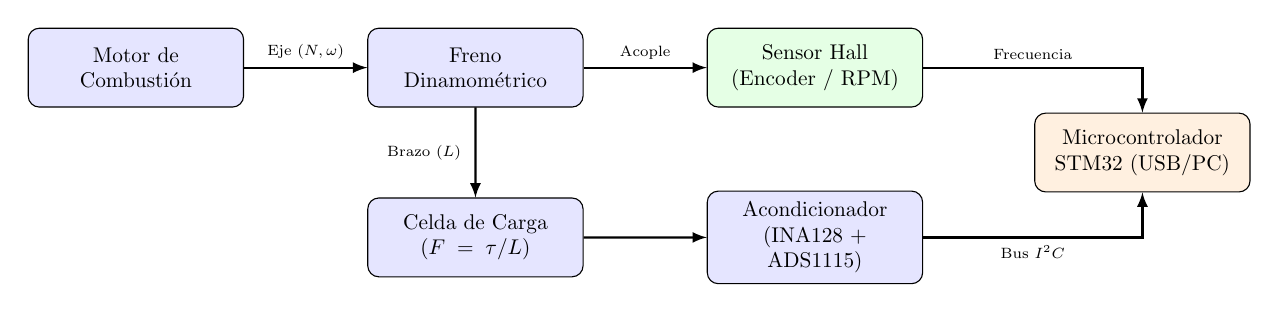
\begin{tikzpicture}[scale=0.77, transform shape,
    block/.style={rectangle, draw, fill=blue!10, text width=3.2cm, text centered,
                  rounded corners, minimum height=1.3cm, inner sep=5pt},
    line/.style={draw, -latex, thick}]

    \node [block] (motor) at (0, 0) {Motor de\\Combustión};
    \node [block] (freno) at (5.6, 0) {Freno\\Dinamométrico};
    \node [block, fill=green!10] (rpm) at (11.2, 0) {Sensor Hall\\(Encoder / RPM)};

    \node [block] (celda) at (5.6, -2.8) {Celda de Carga\\($F = \tau / L$)};
    \node [block] (acond) at (11.2, -2.8) {Acondicionador\\(INA128 + ADS1115)};
    \node [block, fill=orange!12] (mcu)   at (16.6, -1.4) {Microcontrolador\\STM32 (USB/PC)};

    \path [line] (motor) -- node[above, midway, font=\scriptsize] {Eje ($N, \omega$)} (freno);
    \path [line] (freno) -- node[above, midway, font=\scriptsize] {Acople} (rpm);
    \path [line] (freno) -- node[left=3pt, midway, font=\scriptsize] {Brazo ($L$)} (celda);
    \path [line] (celda) -- (acond);
    \path [line] (rpm.east) -- node[above, midway, font=\scriptsize] {Frecuencia} (rpm.east -| mcu.north) -- (mcu.north);
    \path [line] (acond.east) -- node[below, midway, font=\scriptsize] {Bus $\text{I}^2\text{C}$} (acond.east -| mcu.south) -- (mcu.south);
\end{tikzpicture}


    \caption{Diagrama de instrumentación para banco de ensayo dinamométrico de motores.}
    \label{fig.ej2:dinamometro}
\end{figure}




\clearpage
\section{Experimento 3: Perturbaciones Inducidas por la Red Eléctrica (50 Hz)}

Para evidenciar experimentalmente la presencia de las perturbaciones eléctricas de baja frecuencia en el entorno de
laboratorio, se conectó un canal del osciloscopio digital Tektronix TDS 220 a un par de conductores de
aproximadamente $\qty{15}{\centi\meter}$ en circuito abierto, sin conexión a ninguna fuente activa
(ver Figura~\ref{fig.ej3:interferencia_50hz}(a)).

En la Figura~\ref{fig.ej3:interferencia_50hz}(b) se observa la captura en pantalla del osciloscopio. Los parámetros
relevados de forma automática arrojaron:
\begin{itemize}
    \item Frecuencia fundamental medida: $f = \qty{50.20}{\hertz}$ ($T \approx \qty{19.92}{\milli\second}$).
    \item Tensión pico a pico: $V_{pp} = \qty{3.12}{\volt}$ (con escala vertical de $\qty{2.00}{\volt/\text{div}}$).
    \item Tensión eficaz de ciclo: $V_{\text{rms-ciclo}} = \qty{951}{\milli\volt}$.
    \item Base de tiempo: $\qty{10}{\milli\second/\text{div}}$.
\end{itemize}
La forma de onda observada exhibió deformaciones respecto a una senoide pura, atribuibles a la presencia de armónicos
impares inyectados a la red por cargas no lineales. Este ensayo
comprueba que cualquier nodo de alta impedancia no apantallado capta directamente la señal de línea como
tensión de interferencia.

\begin{figure}[!ht]
    \centering
    \begin{subfigure}[t]{0.48\textwidth}
        \centering
        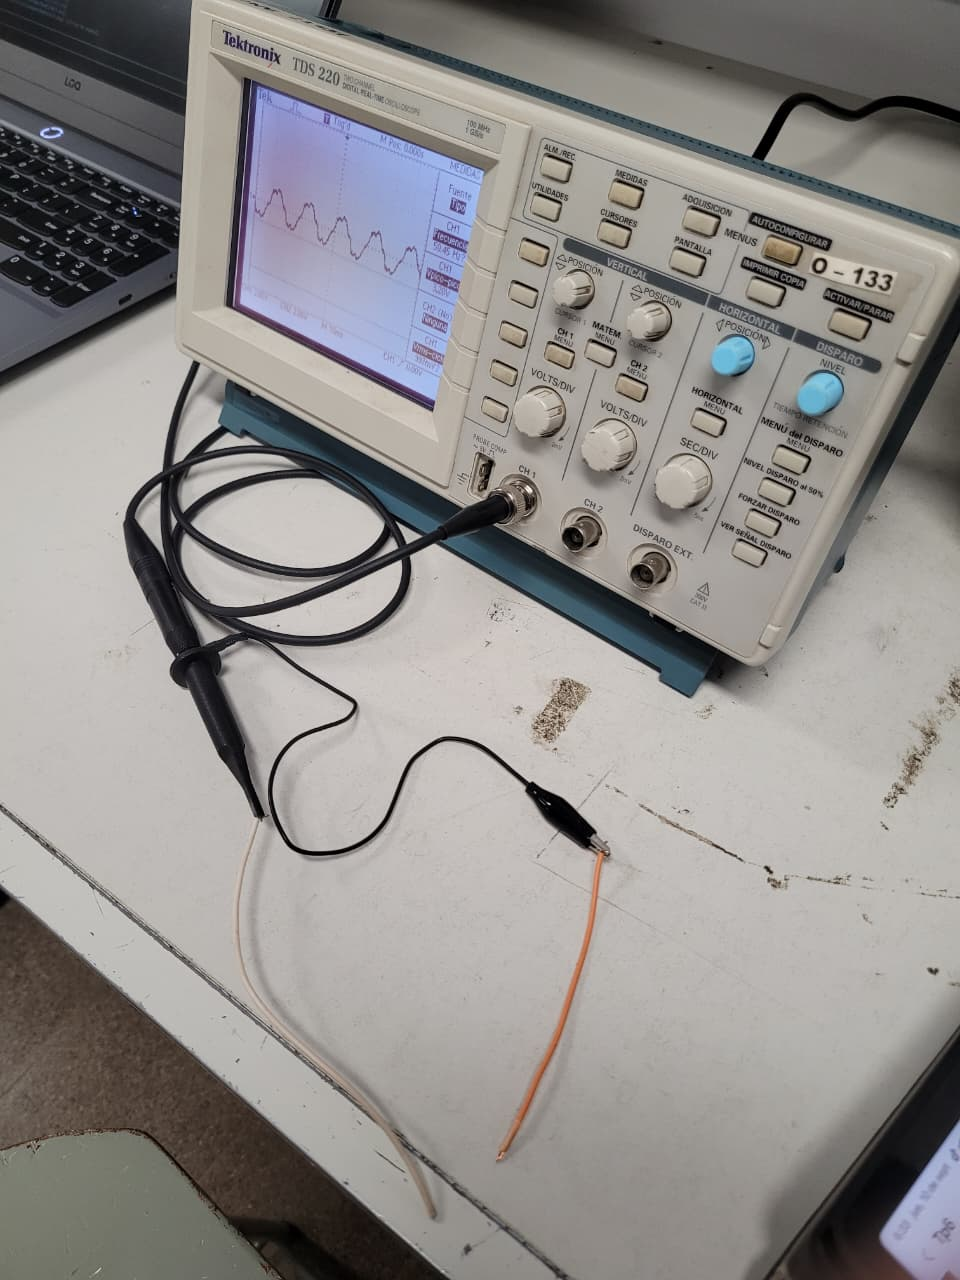
\includegraphics[height=5.8cm, width=\textwidth, keepaspectratio]
        {images/ej3_interferencia_50hz-foto_general.jpeg}
        \caption{Montaje experimental con conductores en circuito abierto.}
        \label{fig.ej3:foto_general}
    \end{subfigure}
    \hfill
    \begin{subfigure}[t]{0.48\textwidth}
        \centering
        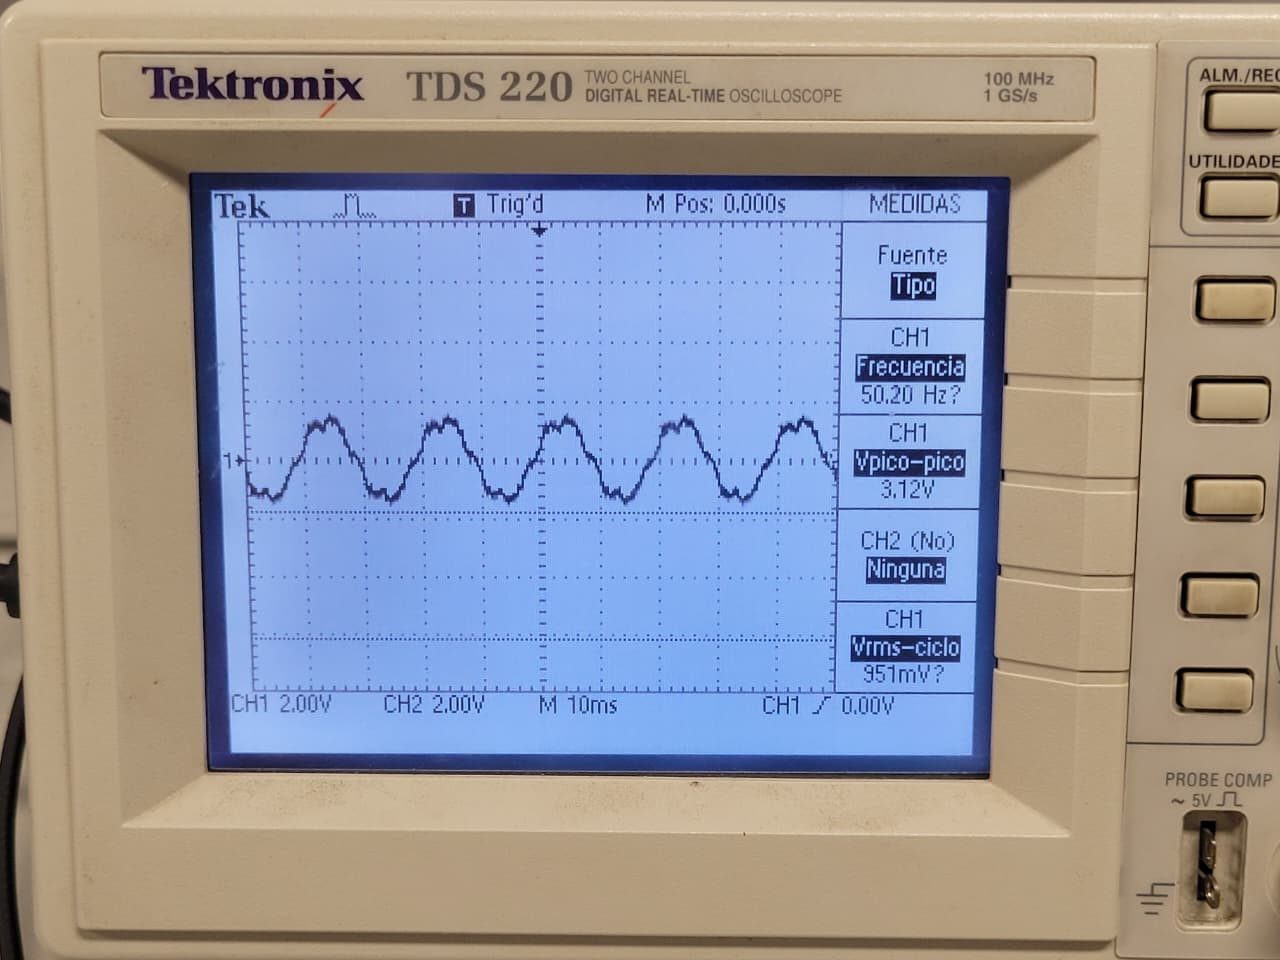
\includegraphics[height=5.8cm, width=\textwidth, keepaspectratio]
        {images/ej3_interferencia_50hz-osc.jpeg}
        \caption{Forma de onda de $\qty{50}{\hertz}$ capturada en el Tektronix TDS 220.}
        \label{fig.ej3:osc_captura}
    \end{subfigure}
    \caption{Medición experimental de perturbaciones inducidas por la red eléctrica comercial ($\qty{50}{\hertz}$).}
    \label{fig.ej3:interferencia_50hz}
\end{figure}

\clearpage
\section{Experimento 4: Medición de Interferencias en Celda de Carga y Técnicas de Blindaje}

\subsection{Medición Directa sobre Celda de Carga sin Acondicionamiento}
Se ensayó inicialmente una celda de carga comercial de $\qty{3}{\kilogram}$ de capacidad nominal. Utilizando el conector
auxiliar provisto en el banco de ensayos, se alimentó el puente de Wheatstone y se midió directamente la salida
diferencial ($V_{\text{in}}^+ - V_{\text{in}}^-$) sin etapa de amplificación intermedia.

Con un multímetro digital en escala de milivoltios de continua se registraron las siguientes tensiones de salida:
\begin{itemize}
    \item En reposo (sin carga): $V_d = \qty{-2.3}{\milli\volt}$ (tensión de desbalance residual de las galgas).
    \item Con una batería (carga patrón a lo largo del experimento) colocada sobre el plato: $V_d = \qty{+7.3}{\milli\volt}$ ($\Delta V_d
        = \qty{9.6}{\milli\volt}$).
\end{itemize}

Al conectar la salida diferencial directamente al canal 1 del osciloscopio en acoplamiento directo (ver
Figura~\ref{fig.ej4:capturas_directa}(a)), se presenta una gran dificultad de apreciar la señal útil. Con una
sensibilidad vertical de $\qty{10.0}{\milli\volt/\text{div}}$ y base de tiempo de $\qty{5.000}{\micro\second/\text{div}}$,
la traza del osciloscopio exhibe un piso de ruido de alta frecuencia con un valor eficaz medido de
$V_{\text{rms}} = \qty{8.57}{\milli\volt}$.

Dado que la excursión total producida por el peso de la batería ($\qty{9.6}{\milli\volt}$) resulta del mismo
orden de magnitud que la tensión de ruido ambiente presente ($\qty{8.57}{\milli\volt}$), la relación señal a
ruido (SNR) es prácticamente unitaria. Esto confirma de modo contundente que resulta inviable digitalizar
directamente la salida de un puente de galgas sin una etapa previa de amplificación diferencial de alta
ganancia, rechazo de modo común y filtrado selectivo.

\subsection{Medición con Placa de Acondicionamiento y Ensayos de Mitigación}
A continuación, se conectó la celda de carga a la placa de acondicionamiento de la cátedra, cuyo circuito esquemático
se detalla en la Figura~\ref{crkt.ej4:banco_celda}. La placa incorpora un amplificador de instrumentación INA122,
polarizado con una fuente externa de $\qty{+9}{\volt}$ regulada localmente a $\qty{+5}{\volt}$ mediante un
regulador lineal para excitar el puente.

\begin{figure}[!ht]
    \centering
    \begin{tikzpicture}[scale=0.85, transform shape]
    % Puente de Wheatstone (Galgas extensométricas)
    \coordinate (top) at (0, 2);
    \coordinate (bottom) at (0, -2);
    \coordinate (left) at (-2, 0);
    \coordinate (right) at (2, 0);

    \draw (top) to[R, l_={$R_1$}] (left)
                to[R, l_={$R_3$}] (bottom)
                to[R, l_={$R_4$}] (right)
                to[R, l_={$R_2$}] (top);

    % Excitación del puente
    \draw (top) to[short, *-o] ++(0, 0.7) node[above] {$V_E$ ($+5\,\unit{\volt}$)};
    \draw (bottom) to[short, *-] ++(0, -0.7) node[ground] {};

    % Malla de cable apantallado (Blindaje / Jaula de Faraday)
    \draw[dashed, red!80!black, thick] (-2.8, 3.6) rectangle (2.8, -3.3);
    \node[red!80!black, font=\footnotesize\bfseries, anchor=south west] at (-2.8, 3.6) {Malla de cable apantallado};
    
    % Conexión a GND de la malla hacia abajo
    \draw[dashed, red!80!black, -latex, thick] (1.5, -3.3) -- ++(0, -0.7);
    \draw (1.5, -4.0) node[ground] {} 
        node[right=4pt, font=\scriptsize, text=red!80!black] {Malla a GND (Conf. 1)};

    % Bloque Amplificador de Instrumentación
    \node[draw, rectangle, minimum width=3.6cm, minimum height=5.0cm, fill=gray!10] (ina) at (8.0, 0) {};
    \node[font=\sffamily\bfseries] at (8.0, 1.7) {INA128 / INA122};

    % Conexiones diferenciales hacia el INA
    % Salida no inversora V+ (nodo derecho del puente) -> Pin 3
    \draw (right) to[short, *-] ++(2.0, 0) |- ([yshift=0.7cm]ina.west);
    \node[anchor=west, font=\scriptsize] at ([xshift=3pt, yshift=0.7cm]ina.west) {Pin 3 ($V_{\text{in}}^+$)};

    % Salida inversora V- (nodo izquierdo del puente) -> Pin 2
    \draw (left) to[short, *-] ++(0, -2.6) -- ++(5.2, 0) |- ([yshift=-0.1cm]ina.west);
    \node[anchor=west, font=\scriptsize] at ([xshift=3pt, yshift=-0.1cm]ina.west) {Pin 2 ($V_{\text{in}}^-$)};

    % Terminales y Resistor de Ganancia RG (Pines 1 y 8)
    \node[anchor=west, font=\scriptsize] at ([xshift=3pt, yshift=-0.9cm]ina.west) {Pin 1 ($R_G$)};
    \node[anchor=west, font=\scriptsize] at ([xshift=3pt, yshift=-1.7cm]ina.west) {Pin 8 ($R_G$)};

    \draw ([yshift=-0.9cm]ina.west) -- ++(-1.0, 0) coordinate (rg_top)
          to[R, l_={$R_G$}] (rg_top |- 0, -1.7)
          -- ([yshift=-1.7cm]ina.west);

    % Alimentación (+5V en Pin 7)
    \draw (ina.north) -- ++(0, 0.6) node[above, font=\scriptsize] {$+5\,\unit{\volt}$ (Pin 7)};

    % Referencia y alimentación negativa (Pines 4 y 5)
    \draw (ina.south) -- ++(0, -0.6) node[ground] {}
          node[right=3pt, font=\scriptsize] {Ref, $-V_S$ (Pines 4, 5)};

    % Salida amplificada (Pin 6)
    \draw (ina.east) to[short, -o] ++(1.2, 0) node[right] {$V_{\text{out}}$ (Pin 6)};
\end{tikzpicture}

    \caption{Circuito esquemático de la placa de acondicionamiento de celda de carga.}
    \label{crkt.ej4:banco_celda}
\end{figure}

Para evaluar la eficacia de las técnicas de apantallamiento y conexión de masa frente a interferencias severas, se
ensayaron tres configuraciones físicas del banco de medición:
\begin{enumerate}
    \item \emph{Configuración 1}: Placa electrónica instalada dentro del gabinete metálico cerrado, con la malla
    conductora del cable blindado conectada a la referencia de potencial 0V (GND).
    \item \emph{Configuración 2}: Placa dentro del gabinete metálico cerrado, pero con la malla conductora del cable
    blindado desconectada (flotante) (ver Figura~\ref{fig.ej4:montajes_ensayo}(a)).
    \item \emph{Configuración 3}: Placa electrónica retirada del gabinete metálico (al aire libre), sin blindaje de
    chasis y con cables sin apantallar (ver Figura~\ref{fig.ej4:montajes_ensayo}(b)).
\end{enumerate}

\begin{figure}[!ht]
    \centering
    \begin{subfigure}[t]{0.48\textwidth}
        \centering
        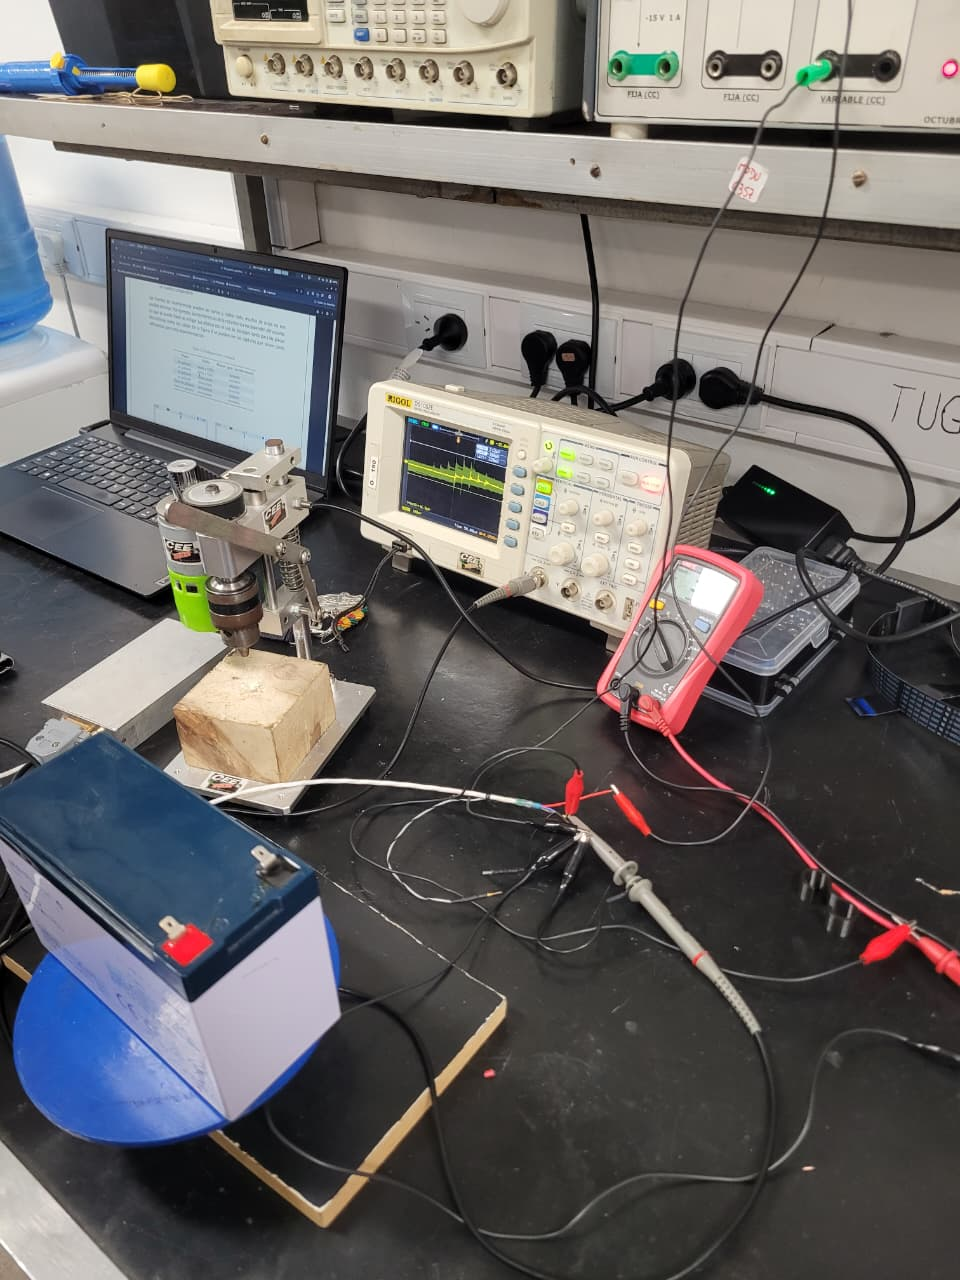
\includegraphics[height=6.2cm, width=\textwidth, keepaspectratio]{images/ej4-blindaje_malla_flotando_sin_motor.jpeg}
        \caption{Banco de ensayo con gabinete metálico y malla flotante (Configuración 2).}
        \label{fig.ej4:montaje_malla_flotante}
    \end{subfigure}
    \hfill
    \begin{subfigure}[t]{0.48\textwidth}
        \centering
        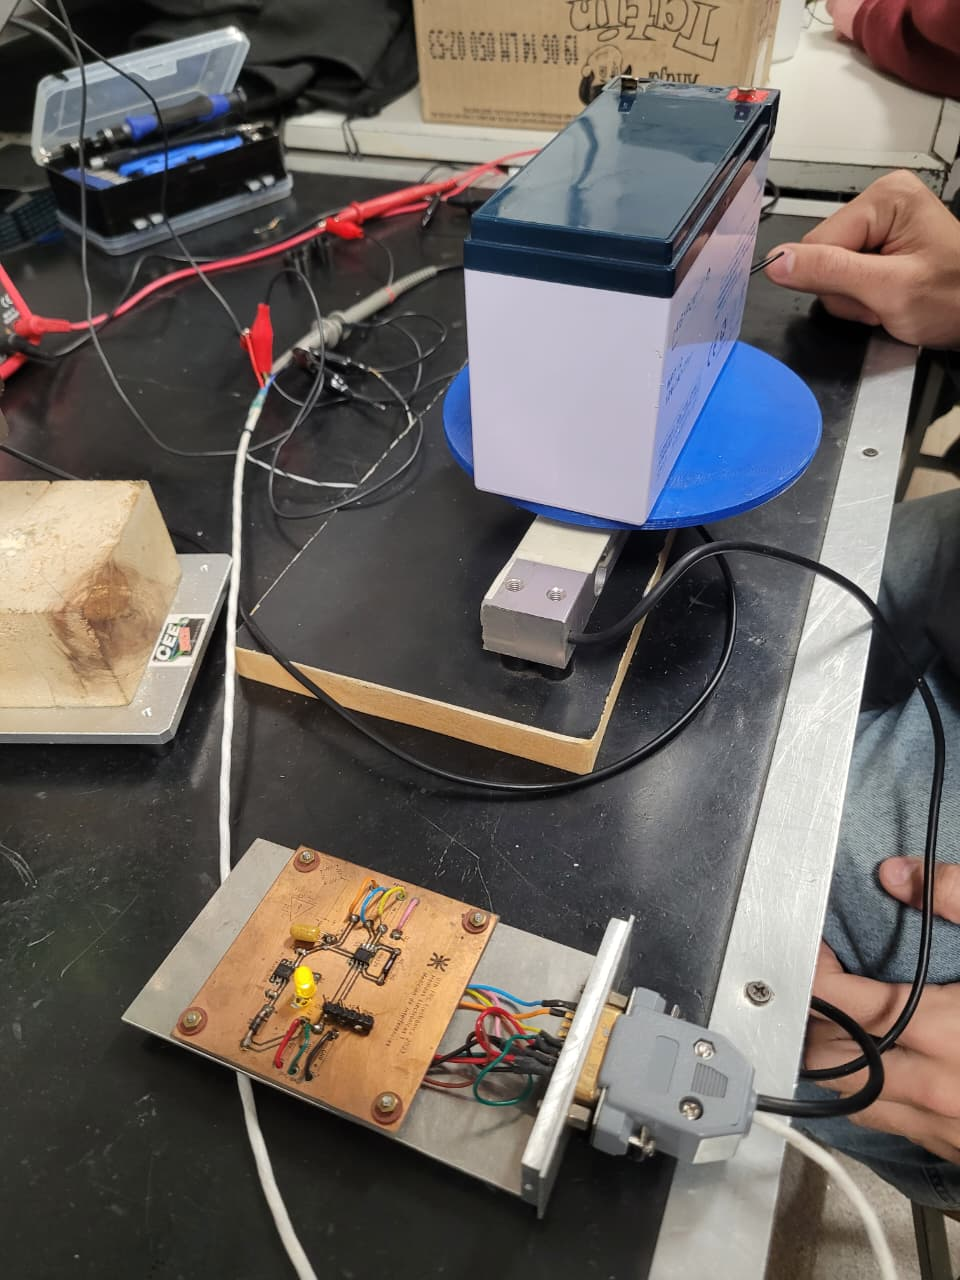
\includegraphics[height=6.2cm, width=\textwidth, keepaspectratio]{images/ej4_medicion_sin_blindaje.jpeg}
        \caption{Placa de acondicionamiento fuera del gabinete y sin blindaje (Configuración 3).}
        \label{fig.ej4:montaje_sin_blindaje}
    \end{subfigure}
    \caption{Montajes experimentales del banco de medición de celda de carga para evaluación de blindajes.}
    \label{fig.ej4:montajes_ensayo}
\end{figure}

Para cada una de las tres configuraciones se realizaron mediciones en dos condiciones de operación:
\begin{itemize}
    \item \emph{En reposo (sin motor)}: En el ambiente estándar del laboratorio central.
    \item \emph{Con perturbación activa (motor Dremel)}: Con un torno manual Dremel encendido y ubicado a
    corta distancia ($\approx \qty{10}{\centi\meter}$) del banco de ensayo, actuando como fuente generadora de
    campos electromagnéticos radiados por arcos de conmutación en su colector de delgas.
\end{itemize}

El osciloscopio se configuró en canal 1 con acoplamiento alterno (CA) y modo de persistencia infinita durante
$\qty{5}{\second}$ para capturar la envolvente total de ruido. Mediante los cursores manuales ($\text{CurA}$ y
$\text{CurB}$) se midió la amplitud pico a pico extrema $\Delta Y = V_{pp}$, el valor eficaz de ruido
$V_{\text{rms}}$ reportado por el instrumento, y la tensión de continua de salida $V_{\text{DC}}$ registrada
simultáneamente con el voltímetro.

\subsection{Resultados Experimentales Obtenidos}
En la Tabla~\ref{tab.ej4:resultados_comparativos} se consolidan de forma sistemática los valores experimentales
obtenidos para las diferentes configuraciones y condiciones de ensayo.

\begin{table}[!ht]
    \centering
    \resizebox{0.95\textwidth}{!}{
    \begin{tabular}{|l|c|c|c|c|}
        \hline
        \textbf{Configuración de Blindaje} & \textbf{Perturbación} &
        \textbf{$V_{\text{DC}}$ [$\unit{\volt}$]} & \textbf{$V_{\text{rms}}$ [$\unit{\milli\volt}$]} &
        \textbf{$V_{pp}$ [$\unit{\volt}$]} \\ \hline
        Conf. 1: En gabinete, malla a GND & Sin motor (Reposo) & 3.45 & 16.0 & 0.204 \\ \hline
        Conf. 1: En gabinete, malla a GND & Con motor Dremel   & 3.93 & 362  & 1.740 \\ \hline
        Conf. 2: En gabinete, malla flotante & Sin motor (Reposo) & 3.39 & 16.5 & 0.320 \\ \hline
        Conf. 2: En gabinete, malla flotante & Con motor Dremel   & 4.13 & 69.3 & 2.160 \\ \hline
        Conf. 3: Sin gabinete, sin malla  & Sin motor (Reposo) & 3.34 & 22.6 & 0.480 \\ \hline
        Conf. 3: Sin gabinete, sin malla  & Con motor Dremel   & 4.14 & 194  & 3.120 \\ \hline
    \end{tabular}}
    \caption{Resultados cuantitativos de ruido e interferencia para las distintas configuraciones.}
    \label{tab.ej4:resultados_comparativos}
\end{table}


En la Figura~\ref{fig.ej4:capturas_directa} se exhiben las pantallas del osciloscopio correspondientes a la señal
directa sin acondicionar y a la condición en reposo. En la Figura~\ref{fig.ej4:capturas_sin_motor} se comparan las
capturas en reposo para las tres configuraciones, y en la Figura~\ref{fig.ej4:capturas_con_motor} se contrastan las
capturas obtenidas bajo la perturbación electromagnética del motor Dremel.

\begin{figure}[!ht]
    \centering
    \begin{subfigure}[t]{0.48\textwidth}
        \centering
        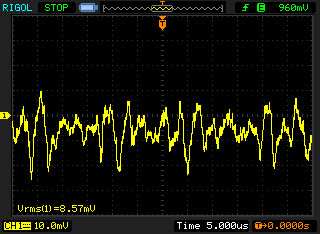
\includegraphics[width=\textwidth]{images/osciloscopio/NewFile9.png}
        \caption{Salida directa de celda sin acondicionar.}
        \label{fig.ej4:dso_directa}
    \end{subfigure}
    \hfill
    \begin{subfigure}[t]{0.48\textwidth}
        \centering
        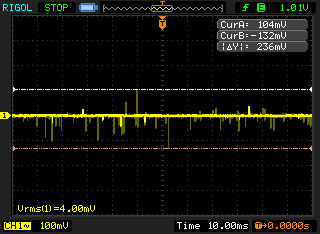
\includegraphics[width=\textwidth]{images/osciloscopio/NewFile10.png}
        \caption{Celda en vacío con acondicionamiento (Conf. 1).}
        \label{fig.ej4:dso_vacio}
    \end{subfigure}
    \caption{Capturas de osciloscopio: señal directa sin acondicionamiento y celda en reposo.}
    \label{fig.ej4:capturas_directa}
\end{figure}

\begin{figure}[!ht]
    \centering
    \begin{subfigure}[t]{0.32\textwidth}
        \centering
        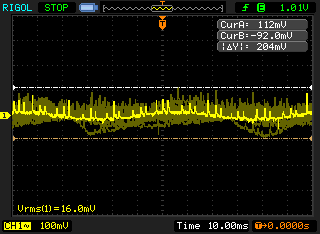
\includegraphics[width=\textwidth]{images/osciloscopio/NewFile11.png}
        \caption{Conf. 1 (malla a GND).}
        \label{fig.ej4:dso_c1_reposo}
    \end{subfigure}
    \hfill
    \begin{subfigure}[t]{0.32\textwidth}
        \centering
        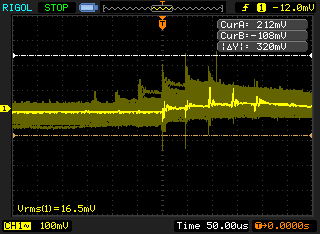
\includegraphics[width=\textwidth]{images/osciloscopio/NewFile13.png}
        \caption{Conf. 2 (malla flotante).}
        \label{fig.ej4:dso_c2_reposo}
    \end{subfigure}
    \hfill
    \begin{subfigure}[t]{0.32\textwidth}
        \centering
        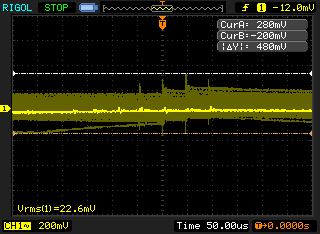
\includegraphics[width=\textwidth]{images/osciloscopio/NewFile15.png}
        \caption{Conf. 3 (sin blindaje).}
        \label{fig.ej4:dso_c3_reposo}
    \end{subfigure}
    \caption{Capturas de persistencia infinita en condición de reposo (sin motor).}
    \label{fig.ej4:capturas_sin_motor}
\end{figure}

\begin{figure}[!ht]
    \centering
    \begin{subfigure}[t]{0.32\textwidth}
        \centering
        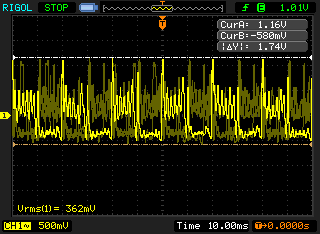
\includegraphics[width=\textwidth]{images/osciloscopio/NewFile12.png}
        \caption{Conf. 1 (malla a GND).}
        \label{fig.ej4:dso_c1_motor}
    \end{subfigure}
    \hfill
    \begin{subfigure}[t]{0.32\textwidth}
        \centering
        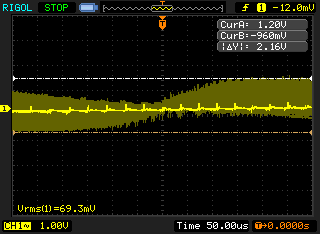
\includegraphics[width=\textwidth]{images/osciloscopio/NewFile14.png}
        \caption{Conf. 2 (malla flotante).}
        \label{fig.ej4:dso_c2_motor}
    \end{subfigure}
    \hfill
    \begin{subfigure}[t]{0.32\textwidth}
        \centering
        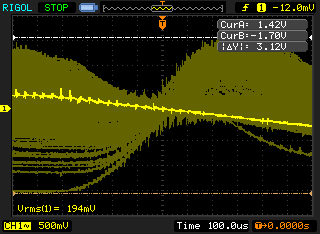
\includegraphics[width=\textwidth]{images/osciloscopio/NewFile16.png}
        \caption{Conf. 3 (sin blindaje).}
        \label{fig.ej4:dso_c3_motor}
    \end{subfigure}
    \caption{Capturas de persistencia infinita bajo perturbación de motor Dremel.}
    \label{fig.ej4:capturas_con_motor}
\end{figure}


Para apreciar claramente la degradación del sistema frente al ruido electromagnético, en la
Figura~\ref{fig.ej4:grafico_ruido} se representa un gráfico de barras comparativo de la tensión de ruido pico a pico
$V_{pp}$ medido mediante cursores.

\begin{figure}[!ht]
    \centering
    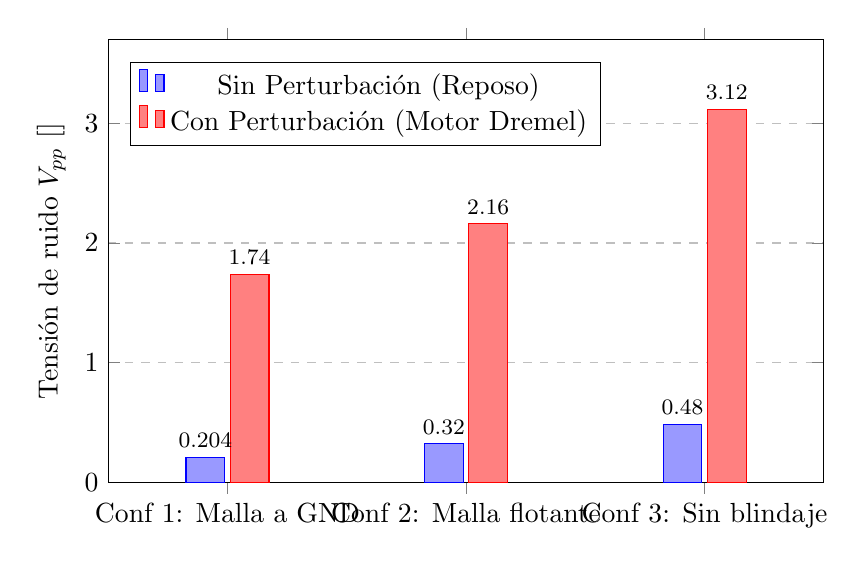
\begin{tikzpicture}
    \begin{axis}[
        ybar,
        bar width=14pt,
        width=0.88\textwidth,
        height=7.2cm,
        ylabel={Tensión de ruido $V_{pp}$ [$\unit{\volt}$]},
        symbolic x coords={Conf 1: Malla a GND, Conf 2: Malla flotante, Conf 3: Sin blindaje},
        xtick=data,
        nodes near coords,
        nodes near coords style={font=\footnotesize, /pgf/number format/fixed, /pgf/number format/precision=3},
        ymin=0,
        ymax=3.7,
        legend style={at={(0.03,0.95)}, anchor=north west},
        ymajorgrids=true,
        grid style=dashed,
        enlarge x limits=0.25
    ]
        \addplot[fill=blue!40, draw=blue] coordinates {
            (Conf 1: Malla a GND, 0.204)
            (Conf 2: Malla flotante, 0.320)
            (Conf 3: Sin blindaje, 0.480)
        };
        \addplot[fill=red!50, draw=red] coordinates {
            (Conf 1: Malla a GND, 1.740)
            (Conf 2: Malla flotante, 2.160)
            (Conf 3: Sin blindaje, 3.120)
        };
        \legend{Sin Perturbación (Reposo), Con Perturbación (Motor Dremel)}
    \end{axis}
\end{tikzpicture}

    \caption{Tensión de ruido pico a pico $V_{pp}$ para las tres configuraciones de blindaje.}
    \label{fig.ej4:grafico_ruido}
\end{figure}

Se puede observar en los ensayos realizados que en condición de reposo (sin motor), la conexión de la
    malla a GND (Configuración 1) permite contener el ruido pico a pico en $\qty{0.204}{\volt}$. Al dejar la
    malla flotando (Configuración 2), el ruido se incrementa a $\qty{0.320}{\volt}$ ($+57\%$), y al eliminar
    totalmente el blindaje (Configuración 3) alcanza $\qty{0.480}{\volt}$ ($+135\%$). Bajo la presencia de la
    perturbación del motor Dremel, la diferencia es aún más notable: la Configuración 1 atenúa el pico de ruido a
    $\qty{1.740}{\volt}$, mientras que la Configuración 2 trepa a $\qty{2.160}{\volt}$ y la Configuración 3
    escala a $\qty{3.120}{\volt}$.

    Por otro lado, se puede confirmar que chasis metálico actúa como blindaje electrostático para las pistas
    del circuito impreso y para el propio circuito integrado. En la Configuración 3, al retirar la placa del gabinete,
    se pudo observar un gran aumento del ruido pico a pico.

